\chapter{Grafos de Kneser}
\label{cap:kneser}

%%%%%%%%%%%%%%%%%%%%%%%%%%%%%%%%%%%%%%%%%%%%%%%
%%% Texto Reescrito
%%%%%%%%%%%%%%%%%%%%%%%%%%%%%%%%%%%%%%%%%%%%%%%

\begin{definicao}
Um grafo de Kneser de parâmetros $n$ e $r$, denotado $KG(n,r)$, é um grafo cujos vértices são todos os $r$-subconjuntos de $[n]$, e dois vértices $v$ e $w$ são adjacentes se $v \cap w = \emptyset$.
\end{definicao}

\begin{figure}[H]
\centering
\begin{tikzpicture}
    \node[anchor=south west,inner sep=0] at (0,0) {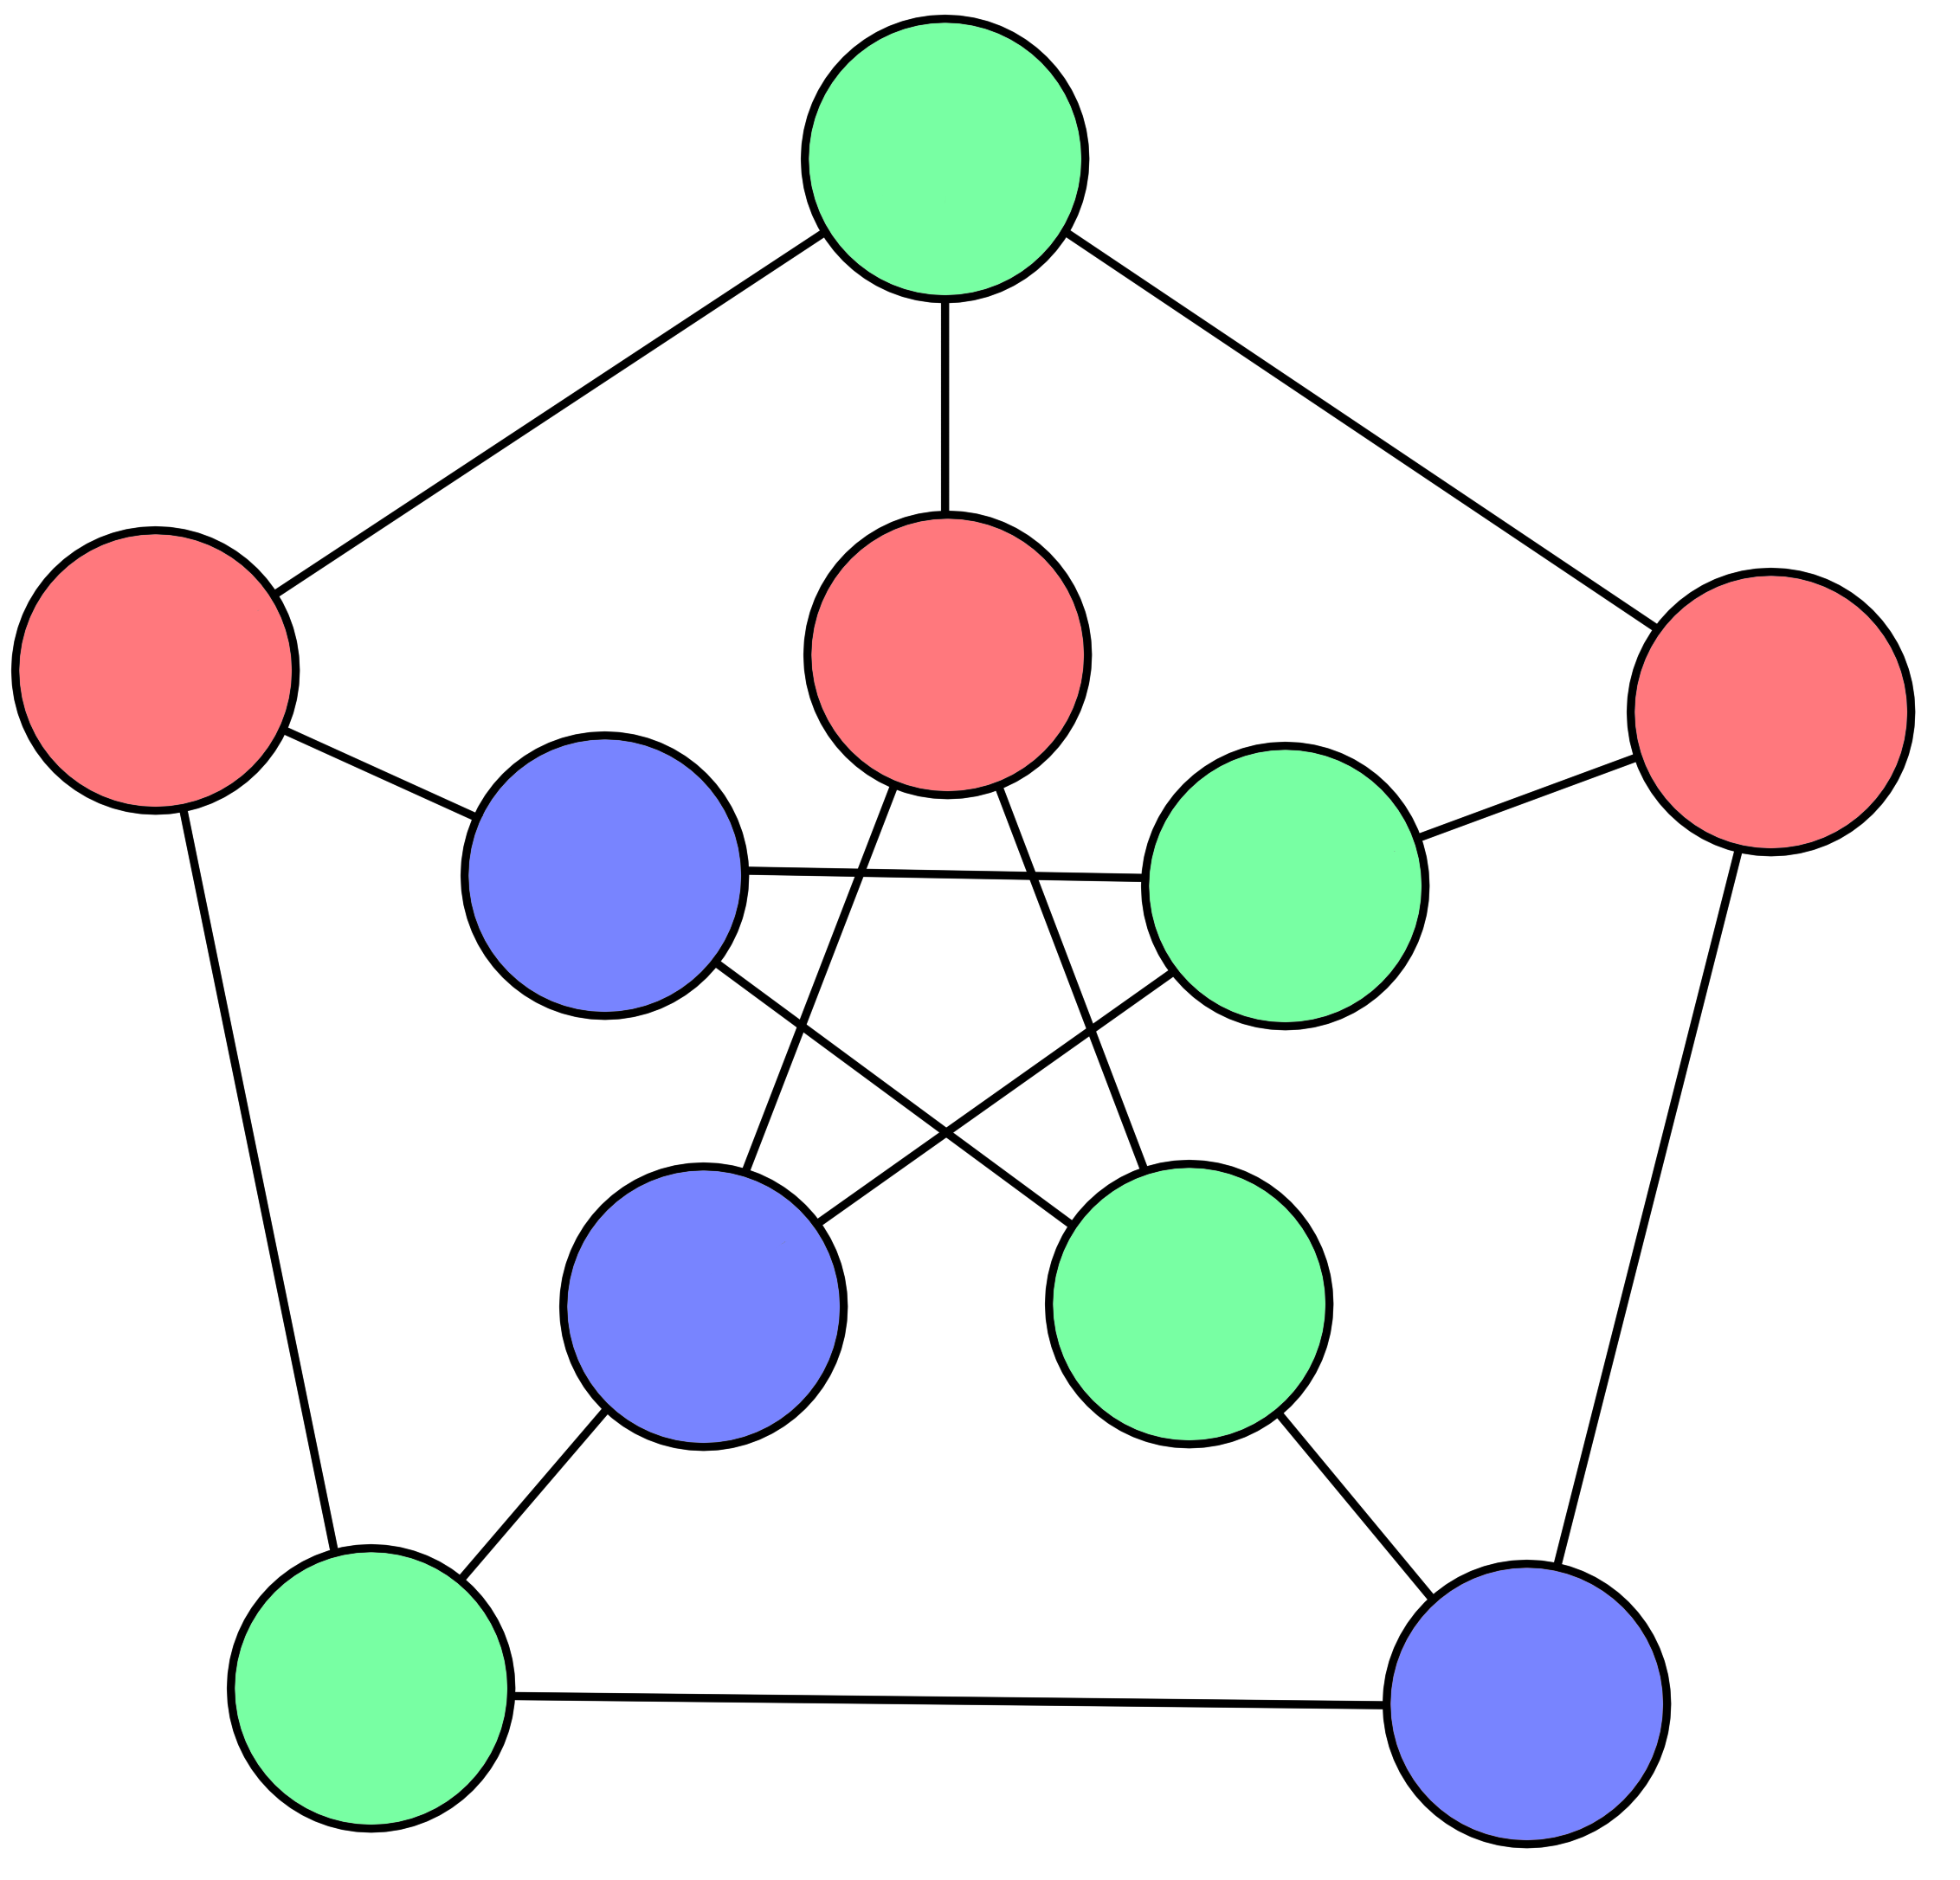
\includegraphics[width=0.5\textwidth]{figuras/ch_kneser/pts-kneser-nt.png}};
    % \draw[red,ultra thick,rounded corners] (7.5,5.3) rectangle (9.4,6.2);
    % \node at (9.55,6.3) {\textbf{texto}};
    \node at (3.95,7.2) {\LARGE$1,2$};
    \node at (3.97,5.1) {\LARGE$3,4$};
    \node at (0.62,5.03) {\LARGE$4,5$};
    \node at (7.45,4.85) {\LARGE$3,5$};
    \node at (2.55,4.2) {\LARGE$2,3$};
    \node at (5.4,4.15) {\LARGE$1,4$};
    \node at (2.95,2.35) {\LARGE$2,5$};
    \node at (5,2.4) {\LARGE$1,5$};
    \node at (1.55,0.8) {\LARGE$1,3$};
    \node at (6.4,0.7) {\LARGE$2,4$};
\end{tikzpicture}
\caption{Grafo de Kneser $KG(5,2)$, isomorfo ao grafo de Petersen.}
\label{fig:kneserpetersen}
\end{figure}

Mohar e Wu demonstraram em \cite{mohar2015triangle} que a conjectura de Erd\H{o}s e Hajnal é verdadeira para os grafos de Kneser.

\begin{definicao}
Seja $G$ um grafo. O \textit{blow-up} de $G$ de potência $m$, denotado por $G^{(m)}$, é um grafo obtido de~$G$ substituindo cada vértice por um conjunto independente de tamanho $m$ (chamado de \textit{blow-up} do vértice), e para cada aresta $xy$ de $G$, o \textit{blow-up} de $x$ e de $y$ formam um grafo bipartido completo $K_{m,m}$. O grafo bipartido completo obtido a partir de uma aresta é chamado de \textit{blow-up} da aresta.
\end{definicao}

\begin{figure}[H]
\centering
\begin{tikzpicture}
    \node[anchor=south west,inner sep=0] at (0,0) {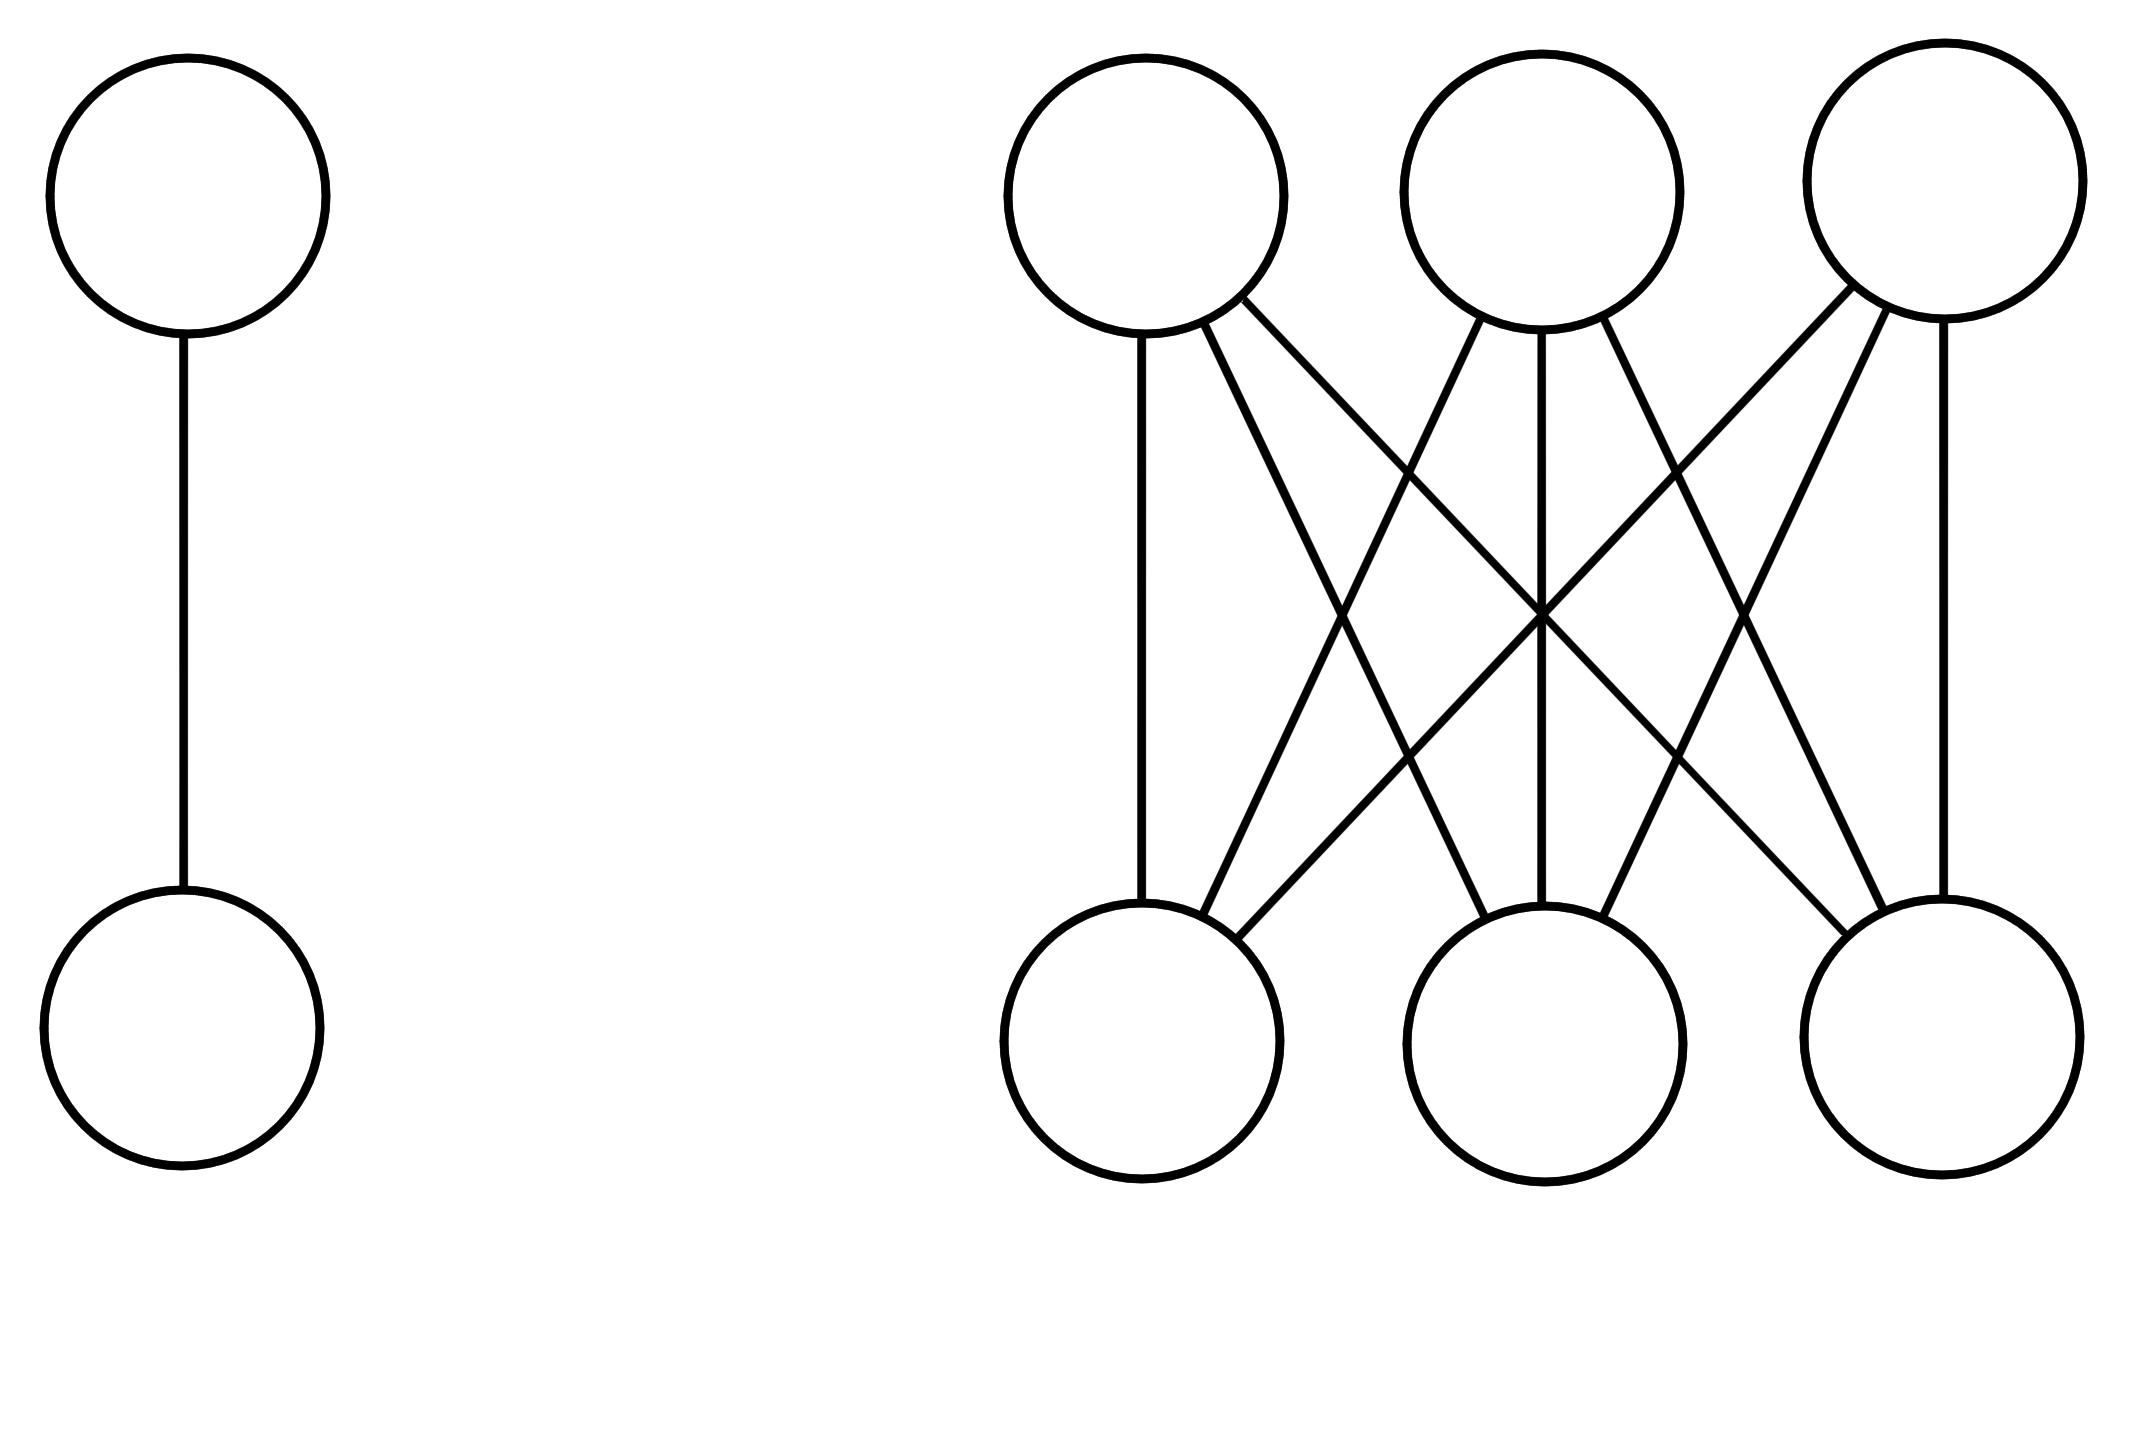
\includegraphics[width=0.5\textwidth]{figuras/ch_kneser/kneser-blowup-nt.png}};
    % \draw[red,ultra thick,rounded corners] (7.5,5.3) rectangle (9.4,6.2);
    % \node at (9.55,6.3) {\textbf{texto}};
    \node at (0.71,4.8) {\LARGE$v$};
    \node at (0.71,1.6) {\LARGE$w$};
    \node at (4.4,4.8) {\LARGE$v_1$};
    \node at (4.4,1.5) {\LARGE$w_1$};
    \node at (5.93,4.8) {\LARGE$v_2$};
    \node at (5.93,1.5) {\LARGE$w_2$};
    \node at (7.46,4.8) {\LARGE$v_3$};
    \node at (7.46,1.5) {\LARGE$w_3$};
    \node at (0.71,0.4) {\LARGE$K_2$};
    \node at (5.93,0.4) {\LARGE$K_2^{(3)}$};
\end{tikzpicture}
\caption{\textit{Blow-up} de $K_2$ de potência $3$.}
\label{fig:kneserblowup}
\end{figure}

\section{Número cromático}

\begin{afirmacao}\label{kneseraffchromatic}
O número cromático de $KG(n,r) = n-2r+2$ se $n\geq 2r$, e $1$ caso contrário.
\end{afirmacao}

Se $n < 2r$, quaisquer dois $r$-subconjuntos de $[n]$ contém um elemento em comum, e logo o grafo $KG(n,r)$ não contém arestas. Portanto $\chi(KG(n,r)) = 1$.

Se $n\geq 2r$, podemos colorir $KG(n,r)$ com $n-2r+2$ cores da seguinte forma, para cada vértice $v$ atribua a cor $\min(v)$ se $\min(v) < n-2r+2$, e caso $\min(v) \geq n-2r+2$, atribua a cor $n-2r+2$. Temos portanto que $\chi(KG(n,r)) \leq n-2r+2$.

Kneser conjecturou que $\chi(KG(n,r)) = n-2r+2$ \cite{kneser1955aufgabe}, e a conjectura foi provada por Lovász \cite{lovasz1978kneser}, por meio do teorema de Borsuk-Ulam \cite{borsuk1933drei}.

\begin{teorema}[Borsuk-Ulam]\label{thborsukulam}
Para toda função contínua $f: S^d \rightarrow\mathbb{R}^d$ da $d$-esfera para o $d$-espaço, existem pontos antípodas $x^*$ e $-x^*$ que são mapeados no mesmo ponto $f(x^*) = f(-x^*)$.
\end{teorema}

A prova será baseada na versão em Aigner e Ziegler \cite{aigner2010proofs}, e faz uso do seguinte seguinte versão do teorema de Borsuk-Ulam, de Greene \cite{greene2002new}.

\begin{teorema}\label{thgreene}
Se a $d$-esfera $S^d$ é coberta por $d+1$ conjuntos $U_1, U_2, \cdots, U_{d+1}$, tal que os primeiros $d$ conjuntos $U_1,\cdots,U_d$ são abertos ou fechados, então algum dos $d+1$ conjuntos contém pontos antípodas $x^*$ e $-x^*$.
\end{teorema}

Seja $d = n - 2r$. Considere $2r+d$ pontos em posição geral na esfera $S^{d+1}$, e seja $V(n,r)$ o conjunto de todos os $r$-subconjuntos dos $2r+d$ pontos na esfera. Suponha que os elementos de $V(n,r)$ estejam particionados em $d+1$ classes, $V(n,r) = V_1 \dot\cup \cdots \dot\cup V_{d+1}$.

Para $i=1,\cdots,d+1$, tome \[O_i = \{x\in S^{d+1} : \text{ O hemisfério aberto } H_x \text{ com polo } x \text{ contém algum } r\text{-conjunto de } V_i\}.\]

\begin{figure}[H]
\centering
\begin{tikzpicture}
    \node[anchor=south west,inner sep=0] at (0,0) {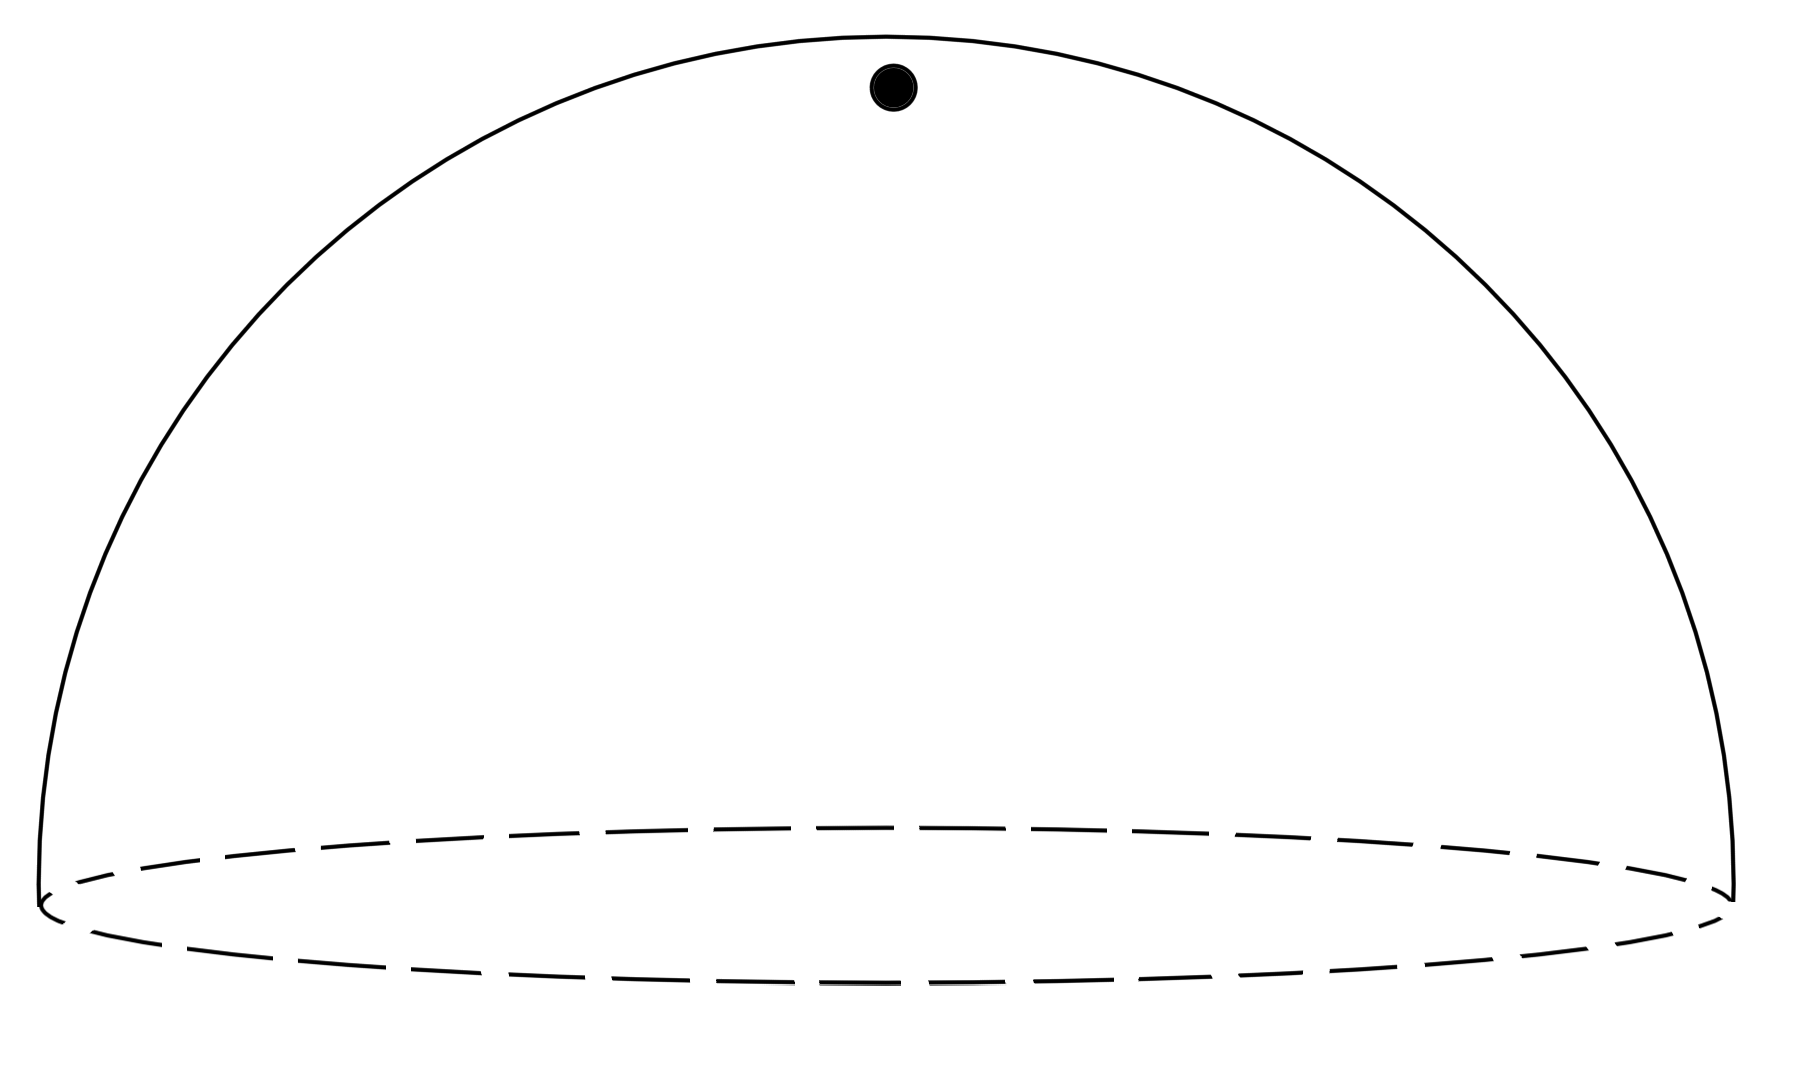
\includegraphics[width=0.45\textwidth]{figuras/ch_kneser/kneser-sphere-hemisphere-nt.png}};
    % \draw[red,ultra thick,rounded corners] (7.5,5.3) rectangle (9.4,6.2);
    % \node at (9.55,6.3) {\textbf{texto}};
    \node at (4.05,3.9) {\LARGE$x$};
\end{tikzpicture}
\caption{Hemisfério aberto $H_x$ em $S^2$.}
\label{fig:kneserhemisphere}
\end{figure}

Note que cada $O_i$ é um conjunto aberto, e o conjunto fechado $C = S^{d+1}\setminus (O_1\cup \cdots \cup O_{d+1})$, junto com os conjuntos $O_i, i=1,\cdots,d+1$ cobrem $S^{d+1}$. Por \ref{thgreene}, algum dos conjuntos $O_i$ ou $C$ contém pontos antípodas $x^*$ e $-x^*$.

Mostraremos que o conjunto $C$ não pode conter pontos antípodas. Suponha que $C$ contenha pontos antípodas $x^*$ e $-x^*$. Pela definição do conjunto $C$, os hemisfério $H_{x^*}$ contém no máximo $r-1$ pontos, pois caso contrário o hemisfério com polo $x^*$ conteria um $r$-conjunto de $V_i$ para algum $i$, e logo $x^* \not\in C$. De mesma forma, o hemisfério $H_{-x^*}$ contém no máximo $r-1$ pontos.

Portanto, temos que pelo menos $n - 2r + 2 = d+2$ pontos estão em $\overline{H_{x^*}}\cap\overline{H_{-x^*}}$, ou seja, $d+2$ pontos estão em um mesmo plano que contém a origem, uma contradição, pois os pontos estão em posição geral.

Portanto, algum conjunto $O_i$ contém pontos antípodas $x^*$ e $-x^*$, e logo existem $r$-conjuntos $A,B \in V_i$, com $A\in H_{x^*}$ e $B\in H_{-x^*}$, e como $H_{x^*}$ e $H_{-x^*}$ são disjuntos, temos que $A$ e $B$ são disjuntos.

\begin{figure}[H]
\centering
\begin{tikzpicture}
    \node[anchor=south west,inner sep=0] at (0,0) {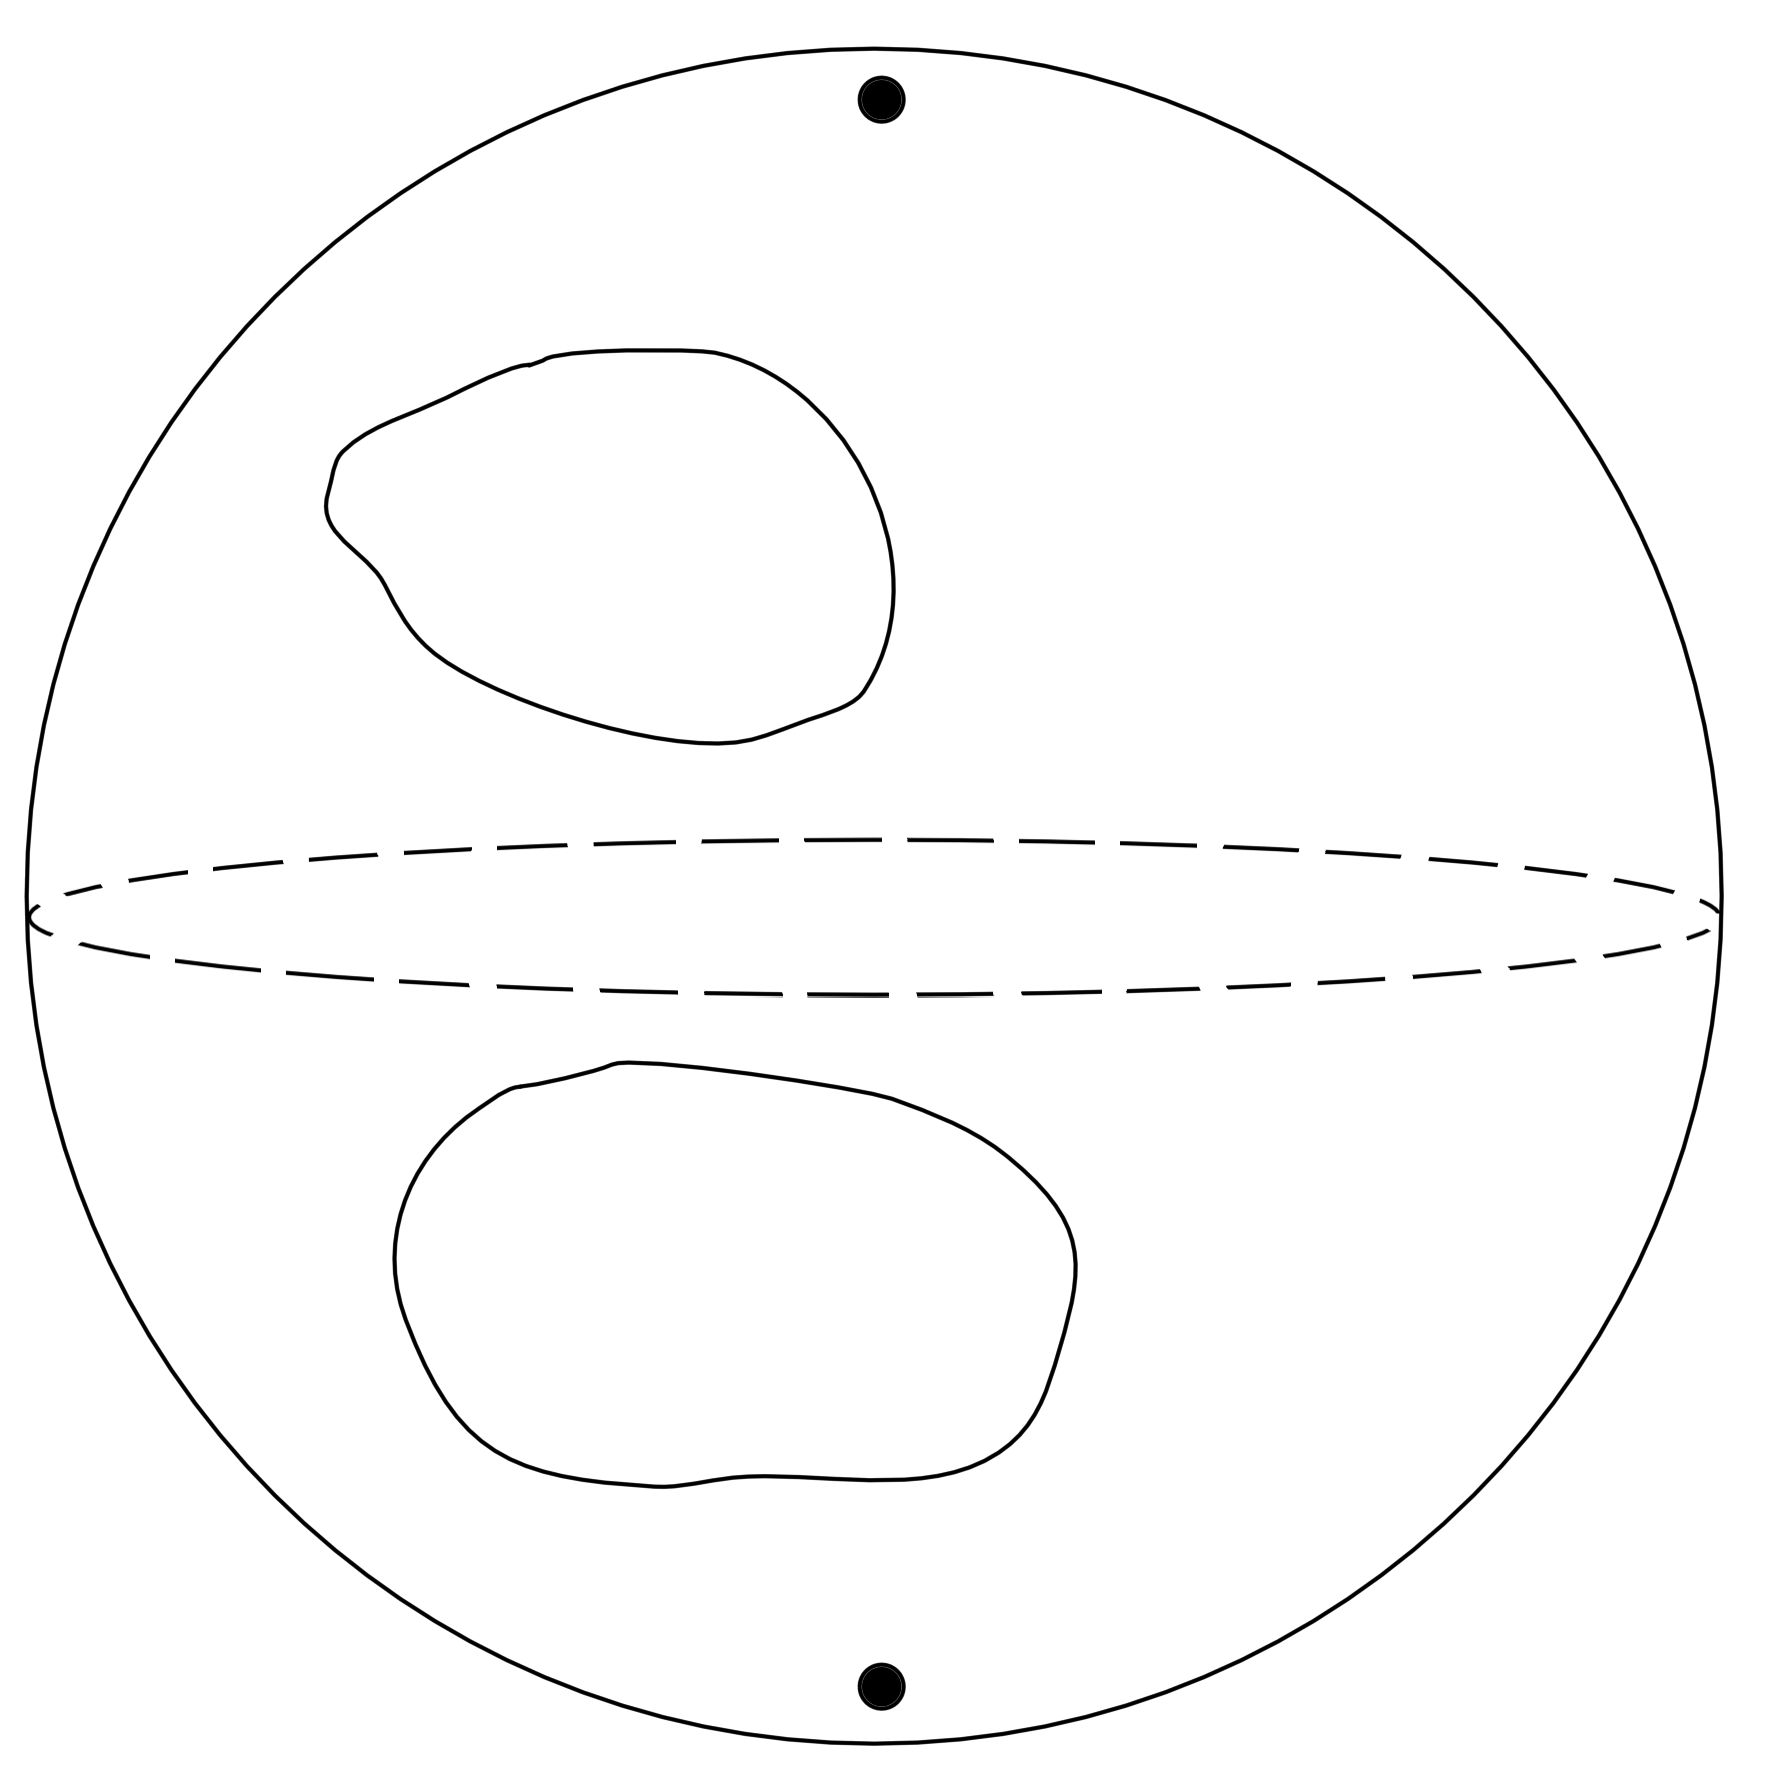
\includegraphics[width=0.4\textwidth]{figuras/ch_kneser/kneser-sphere-AB-nt.png}};
    % \draw[red,ultra thick,rounded corners] (7.5,5.3) rectangle (9.4,6.2);
    % \node at (9.55,6.3) {\textbf{texto}};
    \node at (3.8,5.9) {\LARGE$x^*$};
    \node at (3.8,0.7) {\LARGE$-x^*$};
    \node at (2.3,4.6) {\LARGE$A$};
    \node at (2.75,1.9) {\LARGE$B$};
\end{tikzpicture}
\caption{Hemisférios disjuntos $H_{x^*}$ e $H_{-x^*}$ contendo os $r$-conjuntos $A$ e $B$, respectivamente.}
\label{fig:knesersphereAB}
\end{figure}

% O número cromático de um grafo de Kneser $KG(n,r)$ é $n-2r+2$ se $n \geq 2r$, e $1$ caso contrário \cite{lovasz1978kneser}.

%%%%%%%%%%%%%%%%%%%%
%% Escrever sobre %%
%%%%%%%%%%%%%%%%%%%%

\section{Esboço da Prova}

Mostraremos que se um grafo tem número cromático pelo menos $k$, então um \textit{blow-up} com potência suficientemente grande do grafo contém um subgrafo com cintura grande e número cromático pelo menos $k$.

Mostraremos também que \textit{blow-ups} de grafos de Kneser são subgrafos de grafos de Kneser maiores.

Então, teremos que grafos de Kneser com número cromático suficientemente grande contém \textit{blow-ups} de grafos de Kneser menores, que por sua vez contém um subgrafo com número cromático e cintura grandes.

\section{Prova do Teorema}

Mostraremos então que os grafos de Kneser respeitam a conjectura de Erd\H{o}s e Hajnal.

\begin{teorema}[Mohar e Wu \cite{mohar2015triangle}]\label{moharwuthm}
Suponha que $G$ é um grafo com $\Delta(G) \leq \Delta$ e $\chi(G) \geq k$ para algum $k$. Suponha que $m$ é um inteiro maior que $k(k\Delta)^{2g-4}$. Então existe um subgrafo $H$ de $G^{(m)}$ com cintura maior que $g$ e número cromático maior que $k$.
\end{teorema}

Para demonstrar o Teorema \ref{moharwuthm}, usaremos o seguinte lema.

\begin{lema}\label{lemma1kg}
Dado um grafo $G$ com $\chi(G) > k$, seja $H$ um subgrafo de $G^{(m)}$. Suponha que para toda aresta $ab$ de $G$, e quaisquer subconjuntos $X,Y$ contidos no \textit{blow-up} de $a$ e $b$, respectivamente, com $|X| \geq \frac{m}{k}$ e~$|Y| \geq \frac{m}{k}$, existe uma aresta entre $X$ e $Y$ em $H$. Então $\chi(H) > k$.
\end{lema}

\begin{proof}{(Lema \ref{lemma1kg})} Seja $G$ um grafo com $\chi(G) > k$, e seja $H$ um subgrafo de $G^{(m)}$ tal que para toda aresta $ab$ de $G$ e quaisquer subconjuntos $X,Y$ contidos no \textit{blow-up} de $a$ e $b$, respectivamente, com $|X| \geq \frac{m}{k}$ e $|Y| \geq \frac{m}{k}$, existe uma aresta entre $X$ e $Y$ em $H$. Por simplicidade, suponha que $k$ divide $m$.

Para cada vértice $a$ de $G$, seja $a_H$ o \textit{blow-up} de $a$, ou seja, $a_H$ é o conjunto de $m$ vértices correspondentes ao vértice $a$ em $G^{(m)}$.

Suponha por contradição que $H$ pode ser colorido com até $k$ cores, e fixe uma $k$ coloração de $H$. Como $a_H$ tem $m$ vértices e $H$ pode ser colorido com $k$ cores, pelo princípio da casa dos pombos alguma cor é usada pelo menos $m/k$ vezes em cada $a_H$. Então para cada vértice $a$ de $G$, seja $c(a)$ uma cor que ocorre pelo menos $m/k$ vezes em $a_H$ na coloração fixada.

Para cada aresta $ab$ de $G$, seja $A$ o conjunto de vértices de $a_H$ de cor $c(a)$ e seja $B$ o conjunto de vértices de $b_H$ de cor $c(b)$. Então temos que $|A| \geq m/k$ e $|B| \geq m/k$, e logo pela escolha de $H$, existe uma aresta entre $A$ e $B$. Logo $c(a)$ é diferente de $c(b)$.

\begin{figure}[H]
\centering
\begin{tikzpicture}
    \node[anchor=south west,inner sep=0] at (0,0) {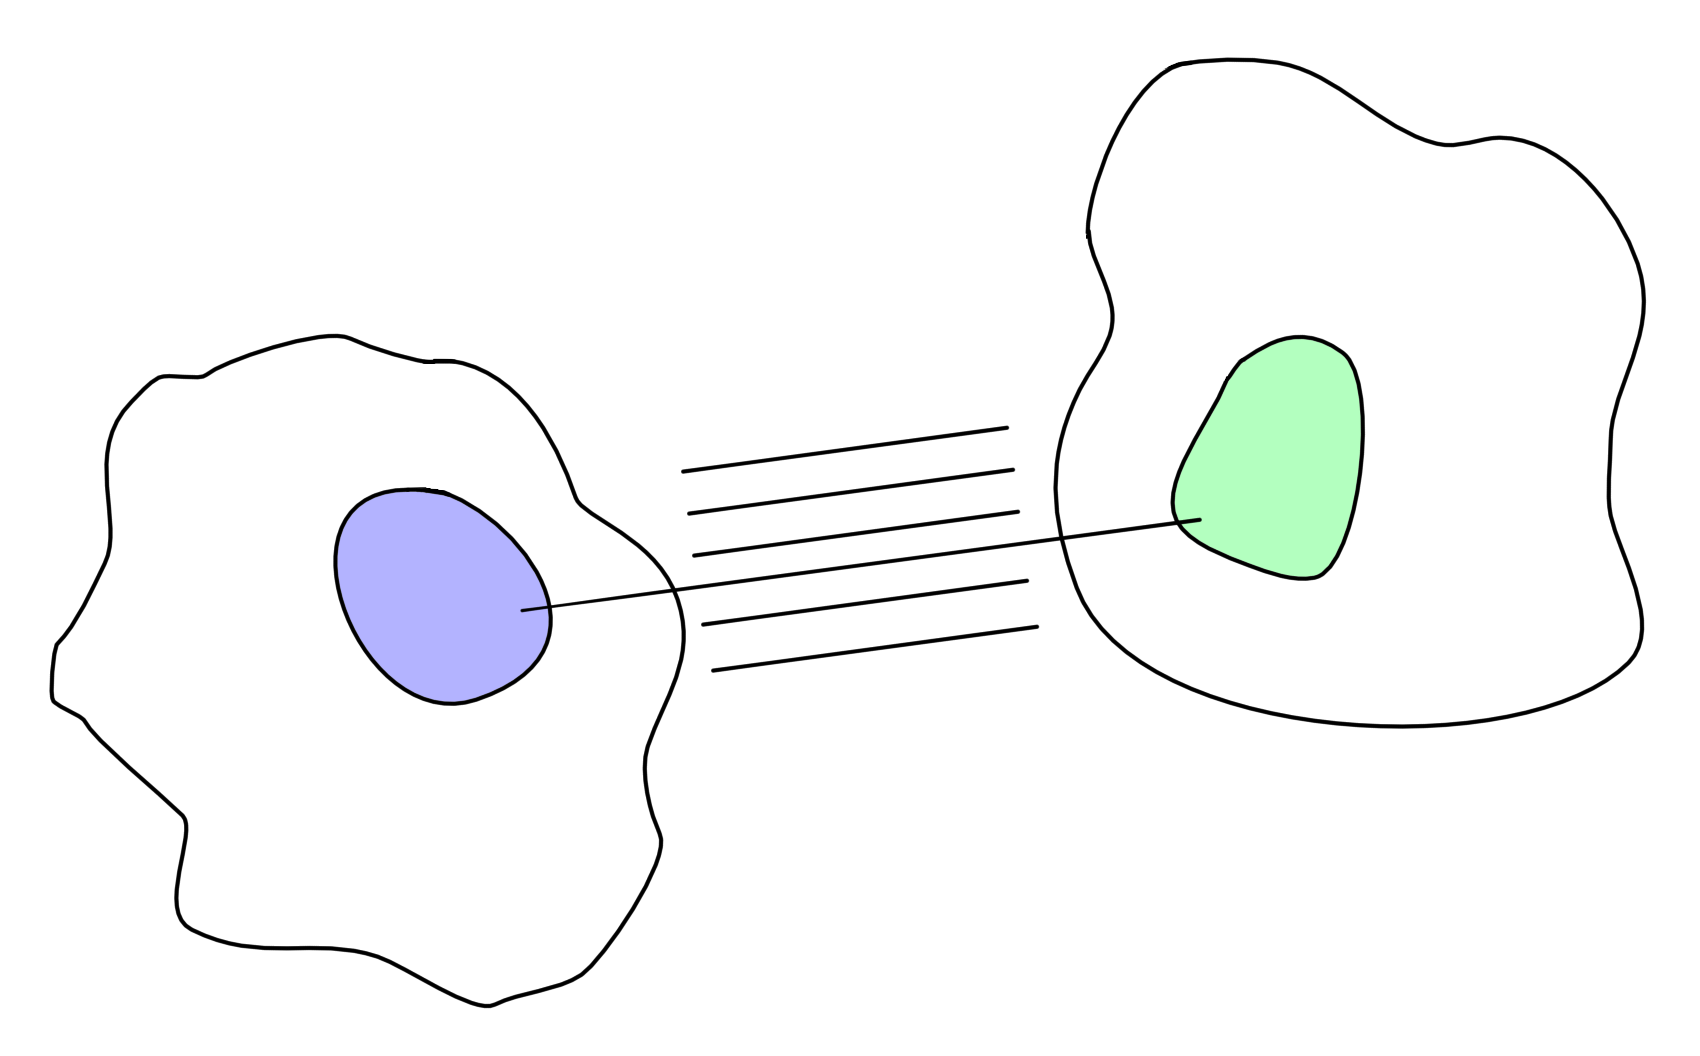
\includegraphics[width=0.6\textwidth]{figuras/ch_kneser/kneser-colorsets-nt.png}};
    % \draw[red,ultra thick,rounded corners] (7.5,5.3) rectangle (9.4,6.2);
    % \node at (9.55,6.3) {\textbf{texto}};
    \node at (2.5,2.65) {\large$\geq$\LARGE{$\frac{m}{k}$}};
    \node at (7.4,3.4) {\large$\geq$\LARGE{$\frac{m}{k}$}};
\end{tikzpicture}
\caption{O \textit{blow-up} de cada vértice contém alguma cor que ocorre pelo menos $m/k$ vezes.}
\label{fig:knesercolorsets}
\end{figure}

Temos portanto que para cada aresta $ab$ de $G$, a cor $c(a)$ é diferente da cor $c(b)$, então podemos colorir cada vértice $a$ de $G$ com a cor $c(a)$ e obteremos uma $k$-coloração de $G$. Contradição, pois $\chi(G) > k$.

Portanto, $H$ não pode ser colorido com apenas $k$ cores.

\end{proof}

\begin{proof}{(Teorema \ref{moharwuthm})}

Seja $s := m/k$, $\lambda := 1/4g$ e $p := s^{\lambda-1}$. Seja $H$ um subgrafo aleatório de $G^{(m)}$, onde cada aresta é escolhida independentemente com probabilidade $p$.

Para cada circuito $C$ de comprimento no máximo $g$ em $G^{(m)}$, seja $A_C$ o evento de todas as arestas de $C$ estarem em $H$. A probabilidade de $A_C$ é a probabilidade de cada aresta de $C$ ser escolhida, portanto temos que $\bbp(A_C) = p^{|C|} = s^{(\lambda-1)|C|}$. Se para todo $C$ vale que $\overline{A_C}$, então a cintura de $H$ é pelo menos $g$.

Seja $B$ um subgrafo do \textit{blow-up} de uma aresta de $G$ isomorfo a $K_{s,s}$. Seja $A_B$ o evento de $H$ não conter nenhuma aresta de $B$. Temos que $\bbp(A_B) = (1-p)^{s^2} \leq e^{-ps^2} = e^{-s^{1+\lambda}}$. Se para todo $B$, vale que $\overline{A_B}$, então para cada aresta $ab$ de $G$ e quaisquer subconjuntos $X,Y$ contidos nos \textit{blow-ups} de $a$ e $b$ respectivamente, com $|X| \geq s$ e $|Y| \geq s$, existe uma aresta entre $X$ e $Y$ em $H$.

Queremos mostrar que existe um subgrafo $H$ de $G^{(m)}$ onde vale $\overline{A_C}$ para todo circuito $C$ com~$|C| \leq g$ e vale $\overline{A_B}$ para todo $B \cong K_{s,s}$. Então mostraremos que

\begin{equation}\label{kneserlllineq}
\bbp\left(\left(\bigwedge\limits_{|C|\leq g}\overline{A_C}\right)\wedge\left(\bigwedge\limits_{B\cong K_{s,s}}\overline{A_B}\right)\right) > 0.
\end{equation}

Mostraremos que (\ref{kneserlllineq}) vale usando o lema local de Lovász.

Para tanto, seja $\mathcal{A}$ a união do conjunto dos eventos $A_C$ para $|C| \leq g$ com o conjunto dos eventos $A_B$ para $B$ isomorfo a $K_{s,s}$. Queremos mostrar que para cada $A\in\mathcal{A}$, existe $y(A) \in (0,1)$ tal que

\[\bbp(A)\leq y(A) \prod_{D\in \Gamma(A)}(1-y(D))\ \forall A\in\mathcal{A},\]

onde $\Gamma(A)$ é o conjunto dos eventos que não são independentes de $A$.

Primeiramente, analisaremos o número de eventos que não são independentes de cada evento~$A_C$ e cada evento $A_B$.

Considere um circuito $C$ com $|C| \leq g$. Como $\Delta(G^{(m)}) \leq m\Delta$, então $C$ compartilha arestas com no máximo $|C|(m\Delta)^{j-2} = |C|(sk\Delta)^{j-2}$ circuitos de comprimento $j$ em $G^{(m)}$, assim como compartilha arestas com no máximo $|C|\binom{m}{s}^2$ cópias de $K_{s,s}$.

Logo cada evento $A_C$ não é independente de no máximo $|C|(sk\Delta)^{j-2}$ outros eventos $A_{C_2}$, onde $C_2$ é um circuito de comprimento $j$, e não é independente de no máximo $|C|\binom{m}{s}^2$ eventos $A_B$ com $B$ isomorfo a $K_{s,s}$.

Considere uma cópia $B$ de $K_{s,s}$. Existem no máximo $s^2(sk\Delta)^{j-2}$ circuitos de comprimento $j$ em $G^{(m)}$ que compartilham arestas com $B$, e existem no máximo $\binom{m}{s}^2$ cópias de $K_{s,s}$ que compartilham arestas com~$B$.

Logo cada evento $A_B$ não é independente de no máximo $s^2(sk\Delta)^{j-2}$ eventos $A_C$ onde $C$ é um circuito de comprimento $j$, e não é independente de no máximo $\binom{m}{s}^2$ eventos $A_{B_2}$, onde $B_2$ é isomorfo a $K_{s,s}$.

Para cada circuito $C$ com $|C| \leq g$, seja $y_{|C|} := y(A_C) = \bbp(A_C)^{1-\lambda} = s^{-(1-\lambda)^2|C|} < s^{(2\lambda - 1)|C|}$, e seja~$y_0 := y(A_B) = e^{-0.5s^{1+\lambda}} \approx \bbp(A_B)^{0.5}$. Então queremos mostrar que

\[\bbp(A_C) \leq y_{|C|}\prod_{D\in\Gamma(A_C)}(1-y(D)),\]
\[\bbp(A_B) \leq y_0\prod_{D\in\Gamma(A_B)}(1-y(D)).\]

Como para cada evento $A$, $y(A) \in (0,1)$, e sabemos um limitante superior para o número de eventos que não são independentes de $A$, temos que

\[\left(\prod_{3\leq j\leq g}(1-y_j)^{|C|(sk\Delta)^{j-2}}\right)(1-y_0)^{|C|\binom{m}{s}^2} \leq \prod_{D\in\Gamma(A_C)}(1-y(D)),\]
\[\left(\prod_{3\leq j\leq g}(1-y_j)^{s^2(sk\Delta)^{j-2}}\right)(1-y_0)^{\binom{m}{s}^2} \leq \prod_{D\in\Gamma(A_B)}(1-y(D)).\]

Então basta mostrar que

\begin{equation}\label{eq1}
\bbp(A_C) \leq y_{|C|}\left(\prod_{3\leq j\leq g}(1-y_j)^{|C|(sk\Delta)^{j-2}}\right)(1-y_0)^{|C|\binom{m}{s}^2},
\end{equation}
\begin{equation}\label{eq2}
\bbp(A_B)\leq y_0 \left(\prod_{3\leq j\leq g}(1-y_j)^{s^2(sk\Delta)^{j-2}}\right)(1-y_0)^{\binom{m}{s}^2}.
\end{equation}

Para simplificar os cálculos, tomaremos o logaritmo das desigualdades.

Primeiramente, consideremos a desigualdade $(\ref{eq1})$. Como $\bbp(A_C) = s^{(\lambda-1)|C|}$, o logaritmo da desigualdade $(\ref{eq1})$ é da forma

\[(\lambda-1)|C|\log(s) \leq \log(y_{|C|}) + \sum_{3\leq j\leq g} |C|(sk\Delta)^{j-2}\log(1-y_j)+|C|\binom{m}{s}^2\log(1-y_0).\]

Como $\log(y_{|C|}) = -(1-\lambda)^2|C|\log(s)$, temos que

\[(\lambda-1)\log(s) \leq -(1-\lambda)^2\log(s)+\sum_{3\leq j\leq g} (sk\Delta)^{j-2}\log(1-y_j)+\binom{m}{s}^2\log(1-y_0).\]

Somando $-(1-\lambda)^2\log(s)$ aos dois lados da inequação, obtemos

\[(\lambda^2 - \lambda)\log(s) \leq \sum_{3\leq j\leq g} (sk\Delta)^{j-2}\log(1-y_j)+\binom{m}{s}^2\log(1-y_0).\]

Por conveniência, podemos multiplicar a inequação por $-1$, e temos

\[(\lambda - \lambda^2)\log(s) \geq -\sum_{3\leq j\leq g} (sk\Delta)^{j-2}\log(1-y_j)-\binom{m}{s}^2\log(1-y_0).\]

Usando o fato de que $0.9\log(1-z) > -z$ para $z>0$ pequeno, temos que $-\log(1-z) < z/0.9$ para $z>0$ pequeno. Então

\[\lambda(1 - \lambda)\log(s) \geq \sum_{3\leq j\leq g} (sk\Delta)^{j-2}\frac{y_j}{0.9}+\binom{m}{s}^2\frac{y_0}{0.9}.\]

Como $y_j = s^{-(1-\lambda)^{2}j}$ e $y_0 = e^{-0.5s^{1+\lambda}}$,

\[0.9\lambda(1 - \lambda)\log(s) \geq \sum_{3\leq j\leq g} (sk\Delta)^{j-2}s^{-(1-\lambda)^2j}+\binom{m}{s}^2e^{-0.5s^{1+\lambda}},\]

e como $s^{-(1-\lambda)^2j} < s^{(2\lambda - 1)j}$, para mostrar que a desigualdade (\ref{eq1}) vale, basta mostrar

\begin{equation}\label{eq3}
0.9\lambda(1-\lambda)\log s \geq \sum_{3\leq j\leq g}s^{(2\lambda-1)j}(sk\Delta)^{j-2}+e^{-0.5s^{1+\lambda}}\binom{sk}{s}^2.
\end{equation}

Agora tome o logaritmo da desigualdade (\ref{eq2}).

\[-s^{1+\lambda} \leq -0.5s^{1+\lambda} + \sum_{3\leq j \leq g} s^2(sk\Delta)^{j-2}\log(1-y_j) + \binom{m}{k}^2\log(1-y_0).\]

De forma semelhante à outra inequação, podemos somar $-0.5s^{1+\lambda}$ aos dois lados da inequação, e multiplicar por $-1$, e obtemos

\[0.5s^{1+\lambda} \geq -\sum_{3\leq j \leq g} s^2(sk\Delta)^{j-2}\log(1-y_j) - \binom{m}{k}^2\log(1-y_0).\]

Como $-\log(1-z) < z/0.9$ para $z>0$ pequeno, temos

\[0.5s^{1+\lambda} \geq \sum_{3\leq j \leq g} s^2(sk\Delta)^{j-2}\frac{y_j}{0.9} + \binom{m}{k}^2\frac{y_0}{0.9},\]

e temos que $y_j = s^{-(1-\lambda)^2j}$ e $y_0 = e^{-0.5s^{1+\lambda}}$, e assim

\[0.45s^{1+\lambda} \geq \sum_{3\leq j \leq g} s^2(sk\Delta)^{j-2} s^{-(1-\lambda)^2j} + \binom{m}{k}^2e^{-0.5s^{1+\lambda}}.\]

Como $s^{-(1-\lambda)^2j} < s^{(2\lambda - 1)j}$, para mostrar que a desigualdade (\ref{eq2}) vale, basta mostrar que

\begin{equation}\label{eq4}
0.4s^{1+\lambda} \geq \sum_{3\leq j\leq g}s^{(2\lambda-1)j}s^2(sk\Delta)^{j-2}+e^{-0.5s^{1+\lambda}}\binom{sk}{s}^2
\end{equation}

Portanto, para provar o Teorema \ref{moharwuthm}, basta mostrar que as desigualdades (\ref{eq3}) e (\ref{eq4}) valem.

Temos o seguinte limitante superior para a somatória da inequação (\ref{eq4})

\begin{equation*}
\setlength{\jot}{5pt}
\begin{aligned}
\sum_{3\leq j\leq g}s^{(2\lambda-1)j}s^2(sk\Delta)^{j-2} & = \sum_{3\leq j\leq g}s^{2\lambda j}(k\Delta)^{j-2} \\
 & \leq s^{2\lambda g}(k\Delta)^{g-2} \\
 & < 1.1s^{2\lambda g}(k\Delta)^{g-2} \\
 & = 1.1s^{0.5}(k\Delta)^{g-2}.
\end{aligned}
\end{equation*}

Como $s = m/k > k(k\Delta)^{2g-4}/k = (k\Delta)^{2g-4}$, temos que $s^{0.5} > (k\Delta)^{g-2}$, e logo temos \\que $1.1s^{0.5}(k\Delta)^{g-2} < 1.1s^{0.5}s^{0.5}$. Portanto,

\begin{equation*}
\sum_{3\leq j\leq g}s^{(2\lambda-1)j}s^2(sk\Delta)^{j-2} < 1.1s.
\end{equation*}

Concluímos também o seguinte limitante superior para a somatória da inequação (\ref{eq3})

\begin{equation*}
\sum_{3\leq j\leq g}s^{(2\lambda-1)j}(sk\Delta)^{j-2} < 1.1s^{-1}.
\end{equation*}

Mostraremos agora um limitante superior para o termo $e^{-0.5s^{1+\lambda}}\binom{sk}{s}^2$, comum às inequações (\ref{eq3}) e (\ref{eq4}).

Como $\binom{sk}{s}^2 < (ek)^{2s}$, temos que

\begin{equation*}
\setlength{\jot}{5pt}
\begin{aligned}
e^{-0.5s^{1+\lambda}}\binom{sk}{s}^2 &< \left(e^{-0.5s^{\lambda}}(ek)^2\right)^s\\
&= \left(e^{-0.5s^\lambda + 2 + 2\log(k)}\right)^s.
\end{aligned}
\end{equation*}

E $s > (k\Delta)^{2g-4}$, logo $s^\lambda > (k\Delta)^{\frac{2g-4}{4g}}$, e como $g \geq 4$, temos que $(k\Delta)^{\frac{2g-4}{4g}} \geq (k\Delta)^{1/4}$. 

Note que como $(k\Delta)^{1/4} > 4(1+\log(k))$ para $k$ suficientemente grande, então

\begin{equation*}
\setlength{\jot}{5pt}
\begin{aligned}
\left(e^{-0.5s^\lambda + 2 + 2\log(k)}\right)^s &< \left(e^{-0.5(4+4\log(k)) + 2 + 2\log(k)}\right)^s\\ 
&= (e^0)^s \\
&= 1.
\end{aligned}
\end{equation*}

Portanto $e^{-0.5s^{1+\lambda}}\binom{sk}{s}^2 < 1$.

Para concluir que as desigualdade \ref{eq3} e \ref{eq4} valem, basta mostrar que

\[0.9\lambda(1-\lambda)\log s \geq 1.1s^{-1} + 1\]
e
\[0.4s^{1+\lambda}\geq 1.1s + 1.\]

Como a ordem de $\log s$ é maior que a ordem de $s^{-1}$, e a ordem de $s^{1+\lambda}$ é maior que a ordem de $s$, as desigualdades valem para $s$ suficientemente grande. E temos que $s$ é grande em função de $k$ e $g$, pois $s > (k\Delta)^{2g-4}$, e $k$ é grande.
\end{proof}

Mostraremos agora que grafos de Kneser contém \textit{blow-ups} de grafos de Kneser menores com potência grande \cite{mohar2016dichromatic}.

\begin{teorema}[Mohar e Wu \cite{mohar2016dichromatic}]\label{moharwukn}
Sejam $n,r,t$ e $x$ inteiros não-negativos tais que $0 < r < n$ e $x < rt$. O grafo de Kneser KG$(nt, rt-x)$ contém o \textit{blow-up} de KG$(n,r)$ com potência $\binom{r(t-1)}{x}$ como subgrafo. Ademais se $x < t$, KG$(nt, rt-x)$ contém o \textit{blow-up} de KG$(n,r)$ com potência $\binom{rt}{x}$, e se $x = t$, contém o \textit{blow-up} de~KG$(n,r)$ com potência $\binom{rt}{x}-r$.
\end{teorema}

\begin{proof}{(Teorema \ref{moharwukn})}
Seja $G = KG(nt, rt-x)$ e $H = KG(n,r)$. Podemos entender os vértices de $G$ como os subconjuntos de tamanho $(rt-x)$ de $[n]\times [t]$, e os vértices de $H$ como os subconjuntos de tamanho~$r$ de $[n]$. 

% \begin{figure}[H]
% \centering
% \includegraphics[width=0.75\textwidth]{figuras/ch_kneser/kneser-knt.png}
% \caption{Um vértice de $G$ (esquerda), e um vértice de $H$ (direita).}
% \label{fig:kneserknt}
% \end{figure}

\begin{figure}[H]
\centering
\begin{tikzpicture}
    \node[anchor=south west,inner sep=0] at (0,0) {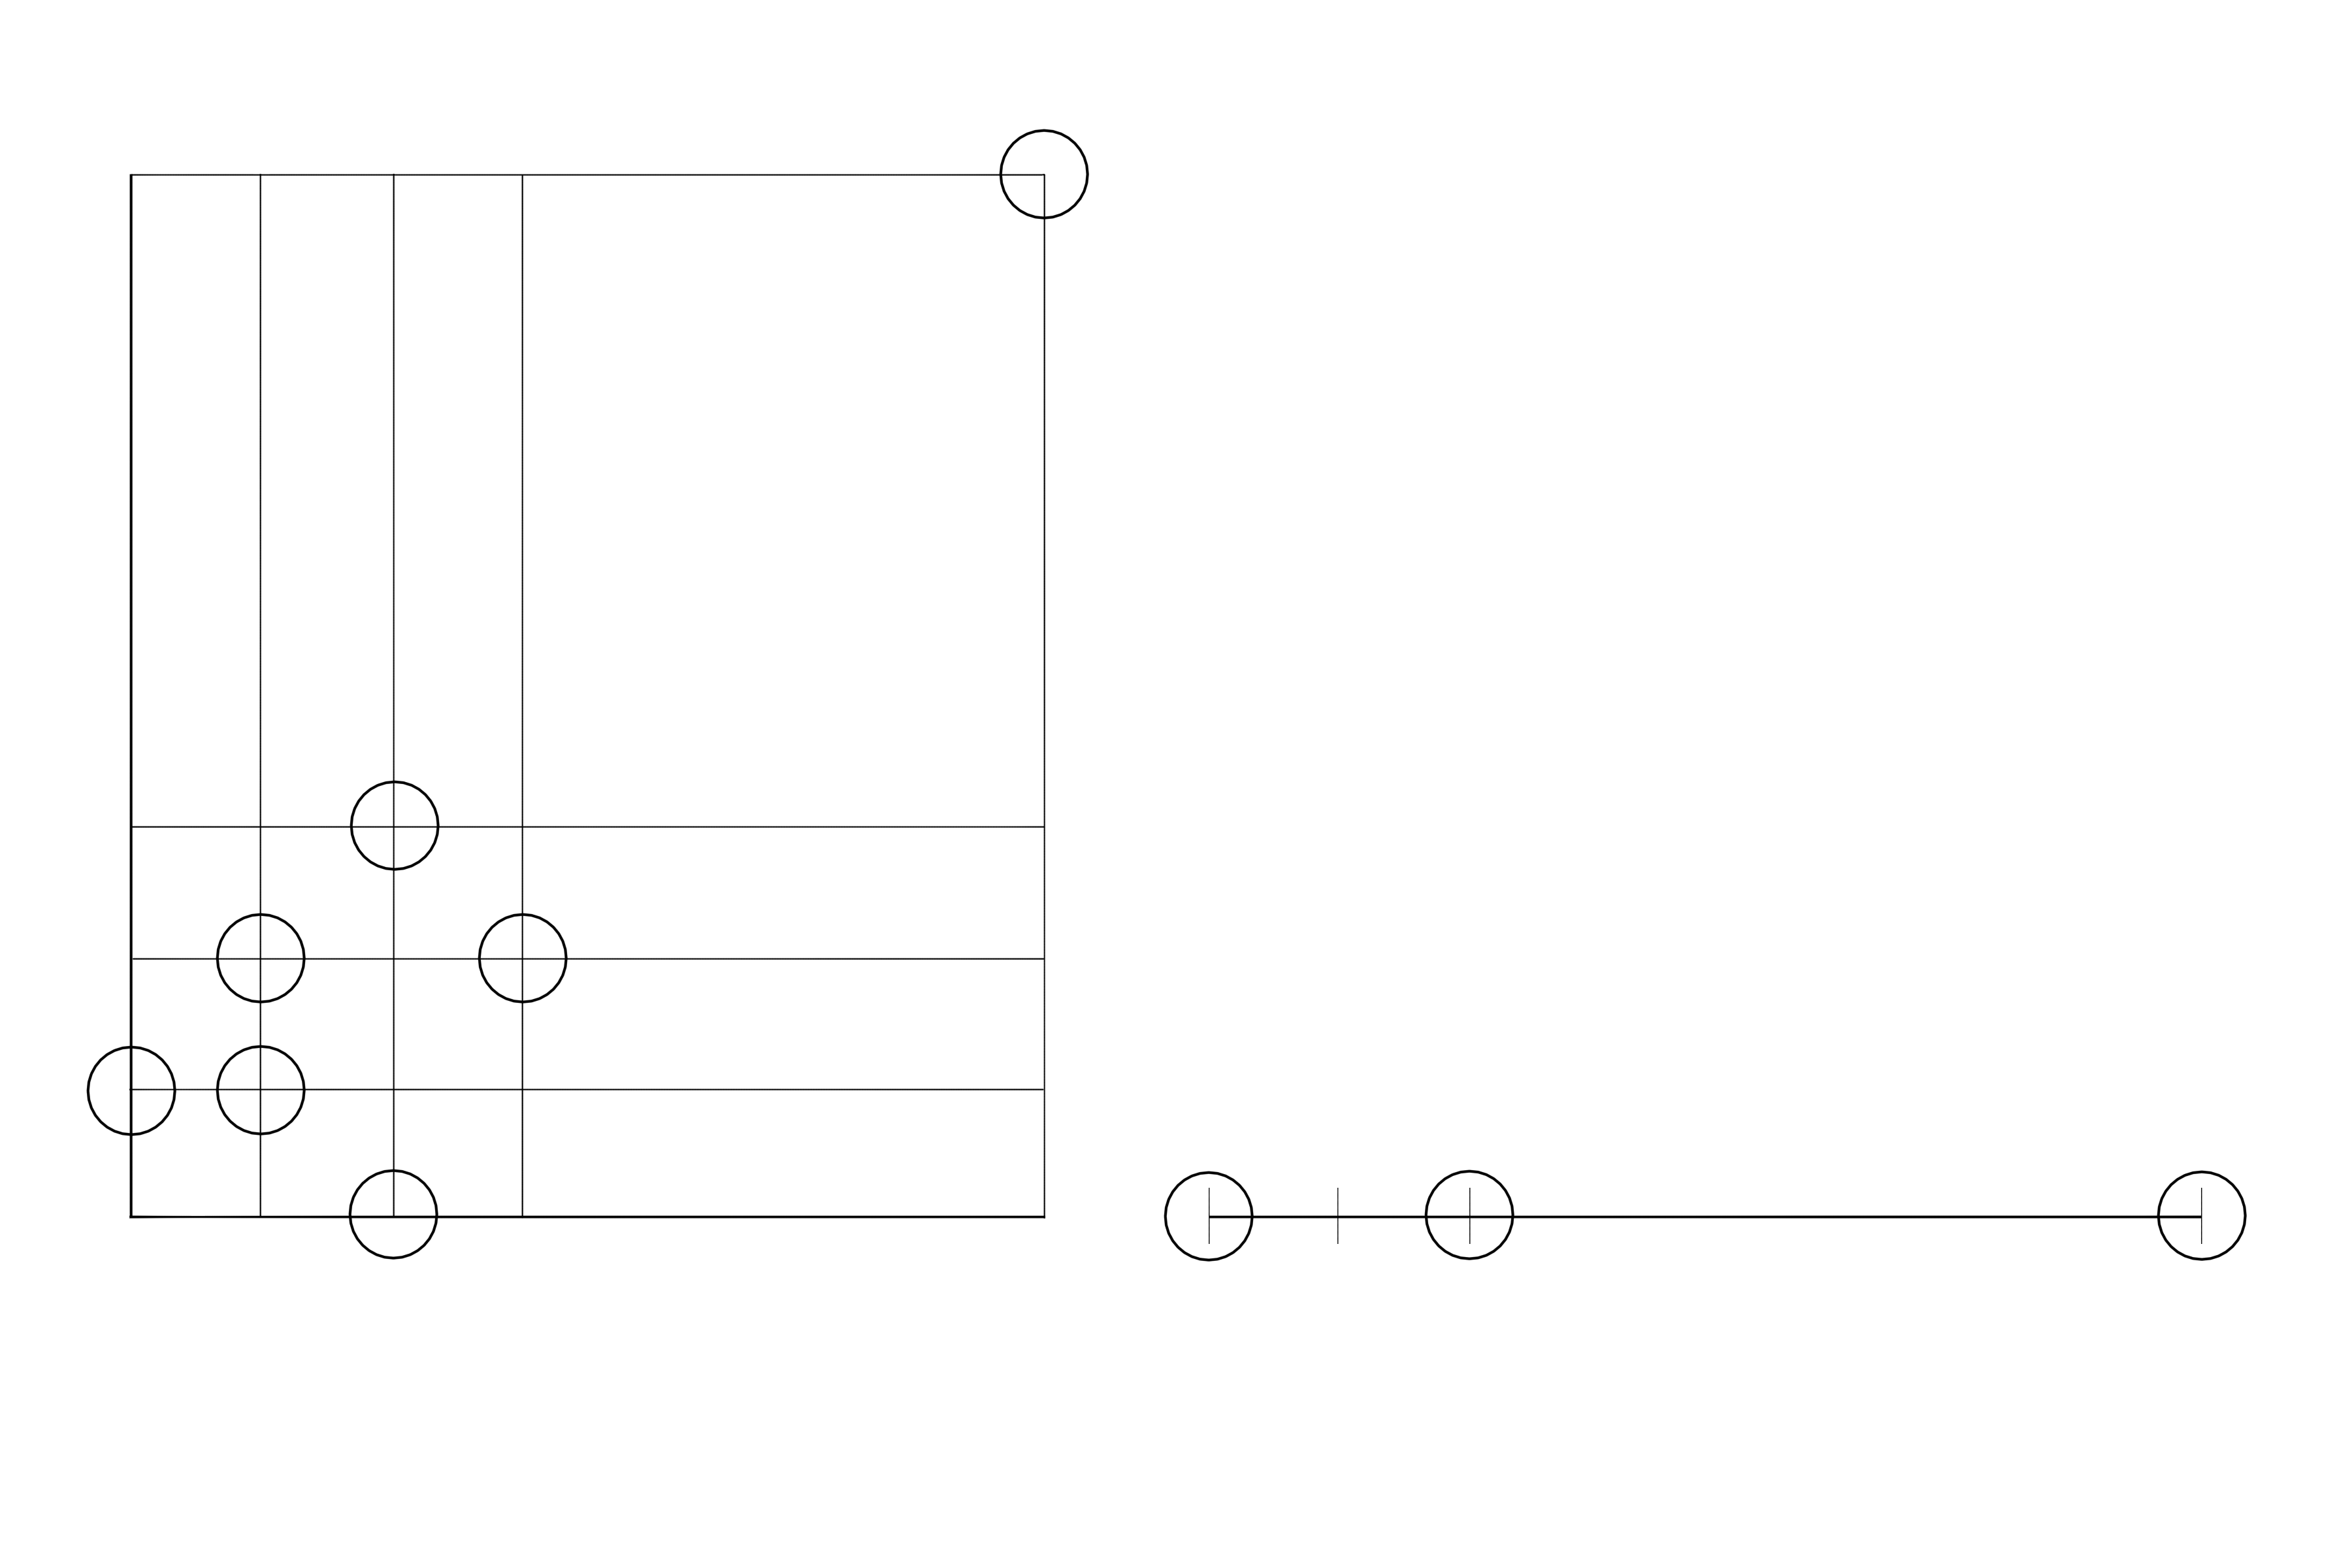
\includegraphics[width=0.75\textwidth]{figuras/ch_kneser/kneser-knt-nt.png}};
    % \draw[red,ultra thick,rounded corners] (7.5,5.3) rectangle (9.4,6.2);
    % \node at (9.55,6.3) {\textbf{texto}};
    \node at (0.65,1.3) {$1$};
    \node at (1.35,1.3) {$2$};
    \node at (2.05,1.3) {$3$};
    \node at (2.75,1.3) {$4$};
    \node at (5.5,1.3) {$n$};
    \node at (6.35,1.3) {$1$};
    \node at (7,1.3) {$2$};
    \node at (7.7,1.3) {$3$};
    \node at (11.6,1.3) {$n$};
    \node at (0.2,1.85) {$1$};
    \node at (0.2,2.5) {$2$};
    \node at (0.2,3.2) {$3$};
    \node at (0.2,3.9) {$4$};
    \node at (0.2,7.3) {$t$};
\end{tikzpicture}
\caption{Um vértice de $G$ (esquerda), e um vértice de $H$ (direita).}
\label{fig:kneserknt}
\end{figure}

Dado um vértice $A\in V(G)$, seja $f(A) = \{a\in [n] : (a,b)\in A \text{ para algum }b\in [t]\}$, ou seja,~$f(A)$ é a projeção de $A$ em $[n]$.

\begin{figure}[H]
\centering
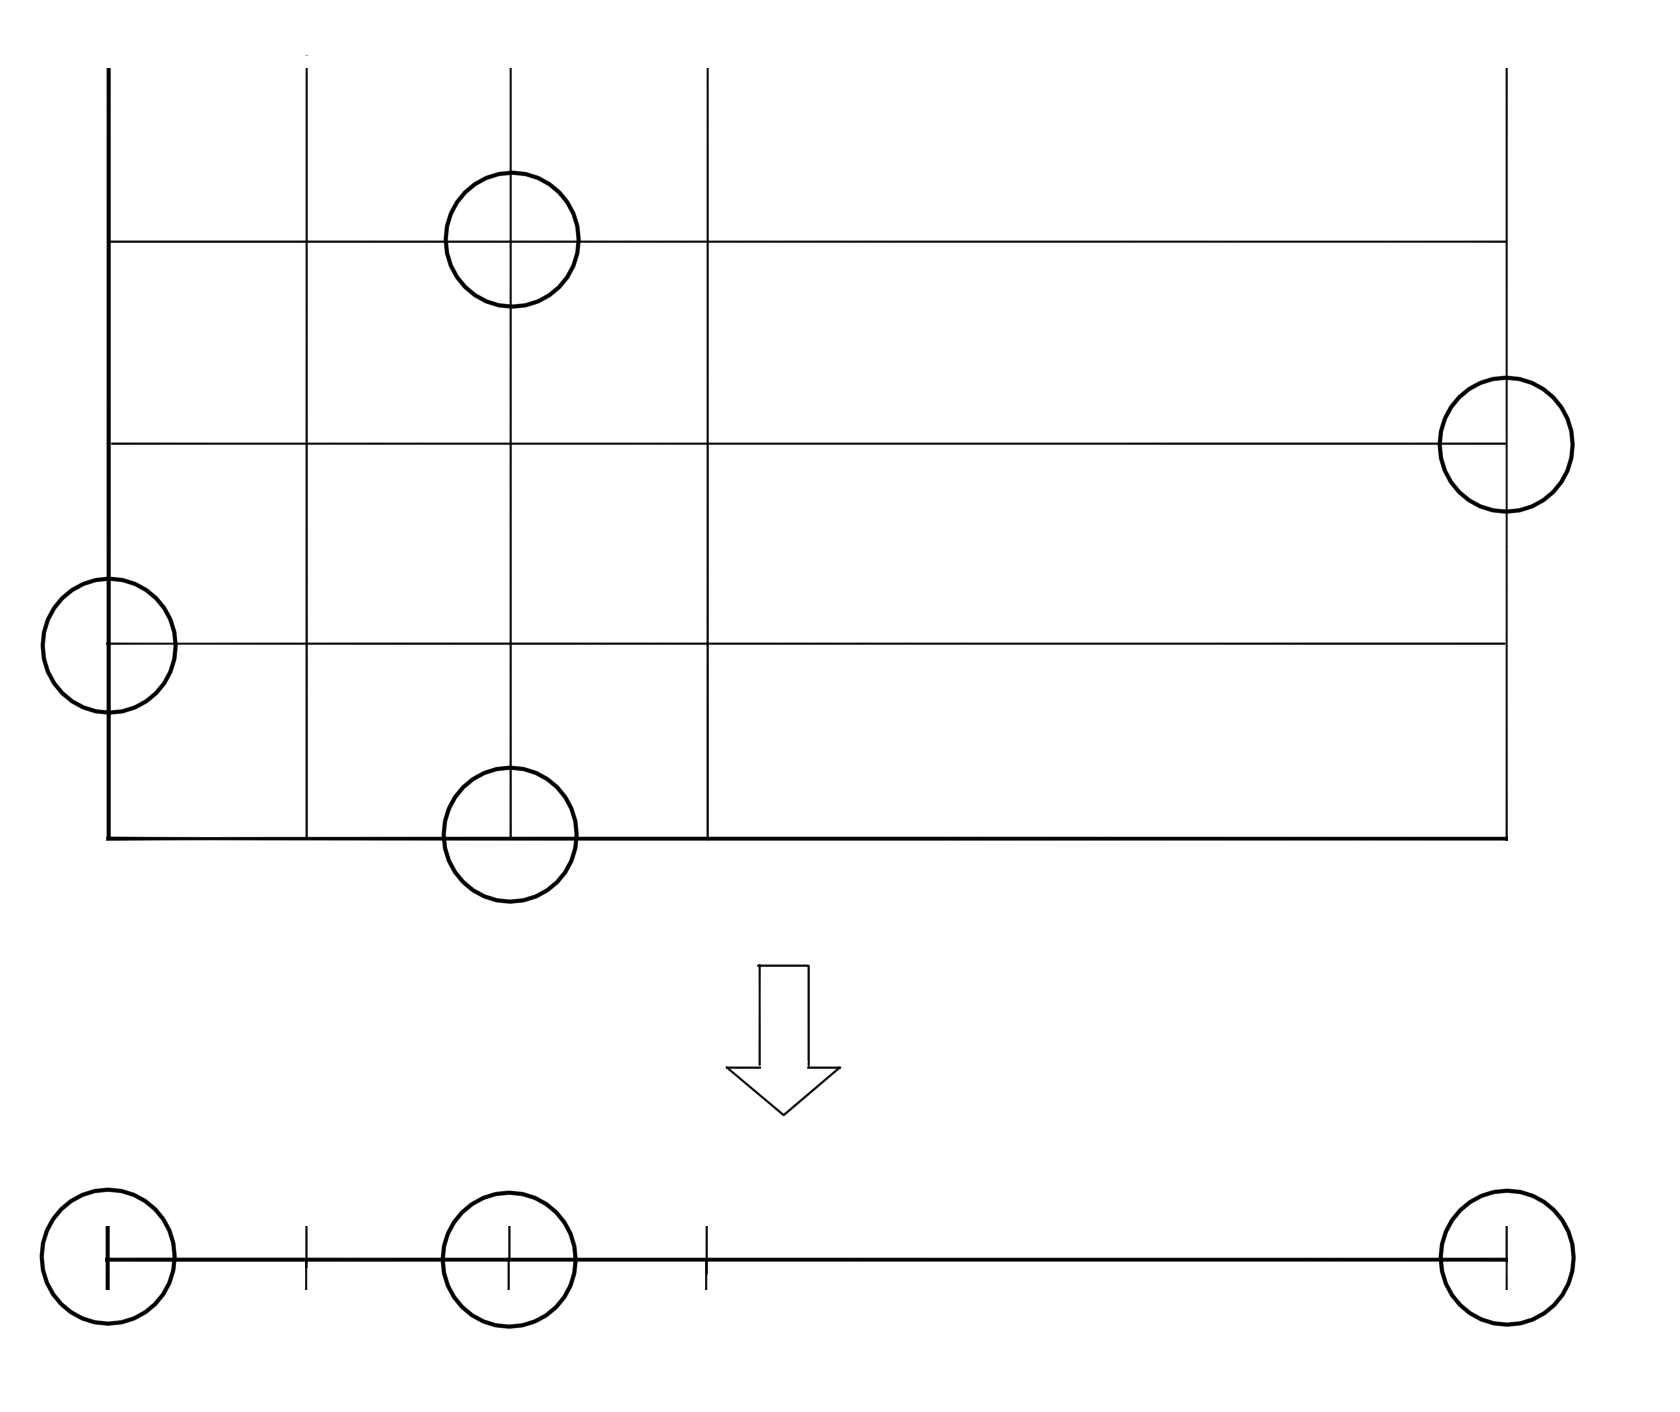
\includegraphics[width=0.5\textwidth]{figuras/ch_kneser/kneser-projection.png}
\caption{Projeção de um vértice de $KG(nt,rt-x)$ em $[n]$.}
\label{fig:kneserprojection}
\end{figure}

Note que se para dois vértices $A,B$ de $G$, temos que $f(A)\cap f(B) = \emptyset$, então $A\cap B = \emptyset$. Logo, se~$|f(A)| = |f(B)| = r$ e $f(A)$ e $f(B)$ são adjacentes em $H$, então $A$ e $B$ são adjacentes em $G$. Para cada vértice $X\in V(H)$, se $f(A) = X$ para algum vértice $A$ de $G$, então $A$ é um subconjunto de $X \times [t]$.

Se $x<t$, como $A \subset X \times [t]$ é um conjunto de tamanho $rt-x$, pelo princípio da casa dos pombos temos que $f(A) = X$. Então existem $\binom{rt}{x}$ vértices de $G$ que são projetados em $X$ por $f$. Temos então que $G$ contém o \textit{blow-up} de $H$ de potência $\binom{rt}{x}$.

Se $x=t$, dentre os possíveis $(rt-x)$-subconjuntos de $X \times [t]$ temos $r$ casos onde $f(A) \neq X$, no caso, os subconjuntos que contém todos os elementos de $(X\setminus v) \times [t]$ para cada $v\in X$. Portanto, temos que $G$ contém o \textit{blow-up} de $H$ de potência $\binom{rt}{x}-r$.

No caso geral, podemos considerar os $(rt-x)$-subconjuntos de $X\times [t]$ que contém todos os elementos de~$X \times \{1\}$. Nesse caso, claramente $f(A) = X$ e temos $\binom{rt-r}{(rt-x)-r} = \binom{r(t-1)}{r(t-1)-x} = \binom{r(t-1)}{x}$ tais subconjuntos. Portanto, $G$ contém o \textit{blow-up} de $H$ de potência $\binom{r(t-1)}{x}$.
\end{proof}

\begin{corolario}\label{knesercor}
A conjectura de Erd\H{o}s e Hajnal é verdadeira para os grafos de Kneser.
\end{corolario}

\begin{proof}{(Corolário \ref{knesercor})}
Sejam $k$ e $g$ os parâmetros da conjectura de Erd\H{o}s e Hajnal, e seja $x$ um inteiro tal que $x \geq 14gk^2\log(k)$ e $x\geq k^4g$. Mostraremos que todo grafo de Kneser da forma $KG(2n, n-2x)$ para algum $n$ contém um subgrafo com número cromático pelo menos $k$ e cintura pelo menos $g$, e com isso, mostraremos que todo grafo de Kneser com número cromático pelo menos $4x+2$ contém um subgrafo com número cromático pelo menos $k$ e cintura pelo menos $g$.

Primeiramente, mostraremos que se supormos que todo grafo de Kneser da forma $KG(2n,n-2x)$ contém um subgrafo com número cromático pelo menos $k$ e cintura pelo menos $g$, então todo grafo de Kneser com número cromático pelo menos $4x+2$ contém um subgrafo com número cromático pelo menos $k$ e cintura pelo menos $g$.

Suponha que $KG(2n,n-2x)$ contém um subgrafo com número cromático pelo menos $k$ e cintura pelo menos $g$. Seja $G_0 = KG(a,b)$ um grafo de Kneser com número cromático pelo menos $4x+2$, e seja $n$ tal que $n-2x = b$. Ou seja, $G_0$ é da forma $KG(a,n-2x)$. Note que $4x+2\leq\chi(G_0) = a-2n+4x+2$, ou seja, temos que $a\geq 2n$.

Se $a = 2n$ então $G_0 = KG(2n,n-2x)$, e portanto contém um subgrafo com número cromático pelo menos $k$ e cintura pelo menos $g$.

Caso contrário temos que $a > 2n$, então basta notar que um grafo de Kneser da forma $KG(a,b)$ contém $KG(a-1,b)$ como subgrafo, e portanto $KG(a,n-2x)$ contém $KG(2n, n-2x)$ como subgrafo, e logo contém um subgrafo com número cromático pelo menos $k$ e cintura pelo menos $g$.

Agora basta provar que $KG(2n,n-2x)$ contém um subgrafo com número cromático pelo menos $k$ e cintura pelo menos $g$.

%Sejam $k$ e $g$ os parâmetros da conjectura de Erd\H{o}s e Hajnal, e seja $G = KG(2n,n-2x)$ um grafo de Kneser com número cromático grande. Claramente $2n \geq 2(n-2x)$, logo temos que $\chi(KG(2n,n-2x)) = 4x+2$.
 

%Sejam $k$ e $g$ os parâmetros da conjectura de Erd\H{o}s e Hajnal, e seja $G = KG(2n,n-2x)$ um grafo de Kneser com número cromático grande. O número cromático de um grafo de Kneser $KG(n,r)$ é igual a $n-2r+2$ se $n \geq 2r$ \cite{lovasz1978kneser}, e $1$ caso contrário, logo para $x\geq 0$ o número cromático de $G$ é $4x+2$. 

Seja $G = KG(2n,n-2x)$ e seja $t = x/k$. Pelo Teorema \ref{moharwukn}, temos que $G$ contém o \textit{blow-up} de $H := KG(2n/t, (n-x)/t)$ com potência~$m = \binom{(n-x)(t-1)/t}{x}$. Por simplicidade, vamos assumir que o resultado das divisões são inteiros. Cada vértice de $H$ tem grau $\binom{(n+x)/t}{(n-x)/t} = \binom{(n+x)/t}{2x/t}$, que é limitado superiormente por

\begin{equation*}
\setlength{\jot}{5pt}
\begin{aligned}
\Delta &:= ((n+x)/t)^{2x/t} \\
&= \left(\frac{nk}{x} + k\right)^{2k}.
\end{aligned}
\end{equation*}

Temos que $G$ contém $H^{(m)}$ como subgrafo. Vamos mostrar que $H^{(m)}$ contém um subgrafo com número cromático pelo menos $k$ e cintura maior que $g$ usando o Teorema \ref{moharwuthm}. Como $\chi(H) = 2k+2$, basta mostrar que $m\geq k(k\Delta)^{2g-4}$.

Consideraremos separadamente dos casos $n > x/(\frac{1}{2} - \frac{1}{2k})$ e $n \leq x/(\frac{1}{2} - \frac{1}{2k})$.

Caso $n > x/(\frac{1}{2} - \frac{1}{2k})$, seja $z$ tal que $\frac{n}{x} = 2 + 2z$. Temos que $z > \frac{1}{k}$, pois

\begin{equation*}
\setlength{\jot}{6pt}
\begin{aligned}
2+2z &= n/x \\
& > \left(\frac{1}{2} - \frac{1}{2k}\right)^{-1}\\
& = \left(\frac{k-1}{2k}\right)^{-1}\\
& = \frac{2k}{k-1}.
\end{aligned}
\end{equation*}

Logo $1+z > k/(k-1) = 1+1/(k-1)$, e portanto $z > 1/(k-1) > 1/k$.

%Como $x \geq 14gk^2\log(k)$, então $x > (k+2)^2$, logo

Temos as três seguintes desigualdades, demonstradas a seguir.

\begin{equation}\label{kncase1eq1}
\frac{n-x}{x}\times \frac{t-1}{t} \geq 1+z.
\end{equation}

\begin{equation}\label{kncase1eq2}
\setlength{\jot}{5pt}
\begin{aligned}
\left(\frac{n}{x}+1\right)^{2k(2g-4)} &= (3+2z)^{2k(2g-4)}\\
&< (1+z)^{x/2}.
\end{aligned}
\end{equation}

%%%%%%%%%%%%%%%%%%%%%%%% Era 10gk^2\log k
%Se $x \geq 14gk^2\log k$, então

\begin{equation}\label{kncase1eq3}
k^{2g(2k+1)} < (1+z)^{x/2}.
\end{equation}

Para mostrar a desigualdade (\ref{kncase1eq1}), temos que

\begin{equation*}
\setlength{\jot}{5pt}
\begin{aligned}
\frac{n-x}{x}\times \frac{t-1}{t} &= \left(\frac{n}{x} - 1\right)\left(1 - \frac{1}{t}\right)\\
&= 1 + 2z - \frac{1+2z}{t}.
\end{aligned}
\end{equation*}

Então, queremos mostrar que

\[1 + 2z - \frac{1+2z}{t} \geq 1 + z,\]

ou equivalentemente, queremos mostrar que

\[z \geq \frac{1+2z}{t}.\]

Como $t,z > 0$, então basta mostrar que 

\[t \geq \frac{1+2z}{z}.\]

Temos que $t = x/k$ e $k > 1/z$, então basta que

\[\frac{x}{k} \geq k + 2.\]

Como $x \geq 14gk^2\log(k)$, então $x/k > k+2$ e logo a desigualdade (\ref{kncase1eq1}) vale.\vspace{1em}

%Para a desigualdade (\ref{kncase1eq2}) temos que $(3+2z)^{2k(2g-4)} < 3^{4kg}(1+z)^{4kg}$, então se $x$ for suficientemente grande em termos de $k$ e $g$, teremos que $3^{4kg}(1+z)^{4kg} < (1+z)^{x/2}$. %% Reescrever

Para a desigualdade (\ref{kncase1eq2}) temos que $(3+2z)^{2k(2g-4)} < (3+3z)^{4kg} = 3^{4kg}(1+z)^{4kg}$, então basta mostrar que \[3^{4kg}(1+z)^{4kg} < (1+z)^{x/2}.\]

Equivalentemente, basta mostrar que  \[3^{4kg} < (1+z)^{x/2 - 4kg}.\]

Como $\frac{1}{k} < z$, temos que \[\left(1+\frac{1}{k}\right)^{x/2-4kg} < (1+z)^{x/2 - 4kg},\]

e como $x\geq 14gk^2\log(k)$, então \[\left(1+\frac{1}{k}\right)^{7gk^2\log(k) - 4kg} \leq \left(1+\frac{1}{k}\right)^{x/2-4kg}.\]

Logo, basta mostrar que

\begin{equation*}
\setlength{\jot}{5pt}
\begin{aligned}
3^{4kg} &<\left(1+\frac{1}{k}\right)^{7gk^2\log(k) - 4kg}\\
&= \left(1+\frac{1}{k}\right)^{kg(7k\log(k)-4)}.
\end{aligned}
\end{equation*}

Equivalentemente, basta mostrar que \[3^4 < \left(1+\frac{1}{k}\right)^{7k\log(k)-4}.\]

%Temos que $1+\frac{1}{k} < 1+z$, pois $\frac{1}{k} < z$, logo $(1+\frac{1}{k})^{x/2-4kg} < (1+z)^{x/2 - 4kg}$. Portanto, basta mostrar que $3^{4kg} < (1+\frac{1}{k})^{x/2-4kg}$.

%Como $x\geq 14gk^2\log(k)$, então $(1+\frac{1}{k})^{7gk^2\log(k) - 4kg} \leq (1+\frac{1}{k})^{x/2-4kg}$. Mostraremos que $3^{4kg} <(1+\frac{1}{k})^{7gk^2\log(k) - 4kg} = (1+\frac{1}{k})^{kg(7k\log(k)-4)}$, equivalentemente mostraremos que $3^4 < (1+\frac{1}{k})^{7k\log(k)-4}$.

Temos que $2k\log(k) > 4$ para $k\geq 2$, então 

\begin{equation*}
\setlength{\jot}{5pt}
\begin{aligned}
\left(1+\frac{1}{k}\right)^{7k\log(k)-4} &> \left(1+\frac{1}{k}\right)^{7k\log(k)-2k\log(k)}\\
&= \left(1+\frac{1}{k}\right)^{5k\log(k)}.
\end{aligned}
\end{equation*}

Note que $(1+\frac{1}{k})^{2k} > e$ para todo $k\geq 1$, logo

\begin{equation*}
\setlength{\jot}{5pt}
\begin{aligned}
\left(1+\frac{1}{k}\right)^{5k\log(k)} &= \left(\left(1+\frac{1}{k}\right)^{2k}\right)^{2.5\log(k)}\\
&> e^{2.5\log(k)}.
\end{aligned}
\end{equation*}

Portanto, basta que $3^4 < e^{2.5\log(k)}$, o que ocorre para todo $k\geq 6$. Portanto a desigualdade (\ref{kncase1eq2}) vale.

%Como $x\geq 14gk^2\log(k)$, basta que $3^{4kg} < (1+z)^{7gk^2\log(k) - 4kg} = (1+z)^{kg(7k\log(k)-4)}$, equivalentemente, podemos escrever $e^{4kg\log(3)} < e^{kg(7k\log(k)-4)\log(1+z)}$. Logo basta mostrar que $4kg\log(3) < kg(7k\log(k)-4)\log(1+z)$, ou seja, que $4\log(3) < (7k\log(k)-4)\log(1+z)$, o que é verdade para $k$ suficientemente grande.\vspace{1em}
%%%%%%%%%%%%%%%%%%%%%%%%%%%%%%%%%%%%%%%%%%%%%%% Isso precisa ser revisto

\vspace{1em}Para a desigualdade (\ref{kncase1eq3}), como $e < (1+1/k)^{k+1}$ para todo $k>0$, temos

\begin{equation*}
\setlength{\jot}{5pt}
\begin{aligned}
k^{2g(2k+1)} & = e^{2g(2k+1)\log k}\\
&< \left(1+\frac{1}{k}\right)^{(k+1)2g(2k+1)\log k}\\
&< \left(1+\frac{1}{k}\right)^{(2k^2+3k+1)2g\log k}.\\
\end{aligned}
\end{equation*}

E como $\frac{1}{k} < z$, temos que \[k^{2g(2k+1)} < \left(1+z\right)^{(2k^2+3k+1)2g\log k}.\]

Para $k \geq 3$, temos que $2k^2+3k+1<3.5k^2$, então 

\begin{equation*}
\setlength{\jot}{5pt}
\begin{aligned}
k^{2g(2k+1)} &< \left(1+z\right)^{(2k^2+3k+1)2g\log k}\\
&< \left(1+z\right)^{(3.5k^2)2g\log k}\\
&= (1+z)^{7gk^2\log k} \\
&\leq (1+z)^{x/2}.
\end{aligned}
\end{equation*}

Portanto a desigualdade (\ref{kncase1eq3}) vale.

Mostraremos que $m \leq k(k\Delta)^{2g-4}$.

%Usando as desigualdades (\ref{kncase1eq1}), (\ref{kncase1eq2}) e (\ref{kncase1eq3}), temos

\begin{equation*}
\setlength{\jot}{5pt}
\begin{aligned}
k(k\Delta)^{2g-4} & = k^{2g-3}\left(\frac{nk}{x}+k\right)^{2k(2g-4)} \\
 & = k^{2g-3}k^{2k(2g-4)}\left(\frac{n}{x}+1\right)^{2k(2g-4)} \\
 & = k^{2g(2k+1) - 8k - 3}\left(\frac{n}{x}+1\right)^{2k(2g-4)}\\
 & < k^{2g(2k+1)}\left(\frac{n}{x}+1\right)^{2k(2g-4)}.
\end{aligned}
\end{equation*}

% \begin{equation*}
% \setlength{\jot}{5pt}
% \begin{aligned}
% k(k\Delta)^{2g-4} & = k^{2g-3}\left(\frac{nk}{x}+k\right)^{2k(2g-4)} \\
%  & = k^{2g-3}k^{2k(2g-4)}\left(\frac{n}{x}+1\right)^{2k(2g-4)} \\
%  & < k^{2g(2k+1)}\left(1+z\right)^{x/2}\\
%  & < (1+z)^{x/2}(1+z)^{x/2} \\
%  & = (1+z)^x \\
%  & \leq \left(\frac{(n-x)(t-1)/t}{x}\right)^x \\
%  & < \binom{(n-x)(t-1)/t}{x} = m.
% \end{aligned}
% \end{equation*}

Pela desigualdade (\ref{kncase1eq2}), temos que \[k^{2g(2k+1)}\left(\frac{n}{x}+1\right)^{2k(2g-4)}< k^{2g(2k+1)}\left(1+z\right)^{x/2}.\]

E pela desigualdade (\ref{kncase1eq1}), temos que \[k^{2g(2k+1)}\left(1+z\right)^{x/2} < (1+z)^{x/2}(1+z)^{x/2}.\]

Logo,

\begin{equation*}
\setlength{\jot}{5pt}
\begin{aligned}
k(k\Delta)^{2g-4} & < (1+z)^{x/2}(1+z)^{x/2} \\
& = (1+z)^x.
\end{aligned}
\end{equation*}

Pela desigualdade (\ref{kncase1eq3}), temos que \[(1+z)^x \leq \left(\frac{(n-x)(t-1)/t}{x}\right)^x.\]

Portanto, temos que

\begin{equation*}
\setlength{\jot}{5pt}
\begin{aligned}
k(k\Delta)^{2g-4} & < \left(\frac{(n-x)(t-1)/t}{x}\right)^x \\
 & \leq \binom{(n-x)(t-1)/t}{x} = m.
\end{aligned}
\end{equation*}

Então $m \leq k(k\Delta)^{2g-4}$, e concluímos o caso $n > x/(\frac{1}{2} - \frac{1}{2k})$.

Caso $n \leq x/(\frac{1}{2} - \frac{1}{2k})$, então $n-2x \leq n/k$. Mostraremos que $KG(2n,n-2x)$ contém $KG(k,1) = K_k$ como subgrafo, e ademais, se $x$ é grande então $KG(2n,n-2x)$ contém um \textit{blow-up} de~$K_k$ com potência grande.

Como $n-2x \leq n/k$, é possível separar $2n$ em $k$ blocos de tamanho $2n/k$, e cada bloco contém pelo menos $n-2x$ elementos. Formalmente, podemos tomar os seguintes conjuntos de vértices.

\[V_i = \left\{v \in V : \ j \in \left[(i-1)\frac{2n}{k}+1, i\frac{2n}{k}\right]\forall j \in v\right\}.\]

Ou seja, cada conjunto $V_i$ contém os vértices formados apenas por elementos de $[(i-1)2n/k+1, i2n/k]$.

Logo cada conjunto corresponde a $\binom{2n/k}{n-2x}$ vértices de $KG(2n, n-2x)$, e vértices de blocos distintos são adjacentes, pois seus conjuntos claramente tem interseção vazia.

Então temos $k$ conjuntos de vértices, cada conjunto com $m := \binom{2n/k}{n-2x}$ vértices, e todo par de vértices de conjuntos distintos são adjacentes. Portanto temos um \textit{blow-up} de $K_k$ com potência $m$.

Se $m \geq k(k\Delta)^{2g-4}$, onde $\Delta := \Delta(K_k) = k-1$, então pelo Teorema \ref{moharwuthm} o \textit{blow-up} de $K_k$ com potência $m$ contém um subgrafo com número cromático pelo menos $k$ e cintura pelo menos $g$.

Portanto basta mostrar que para $x$ suficientemente grande, vale que $m \geq k(k\Delta)^{2g-4}$.

Temos que $x\geq k^{4g}$. É razoável supor que $n-2x > 0$. Então

\begin{equation*}
\setlength{\jot}{5pt}
\begin{aligned}
m &= \binom{2n/k}{n-2x}\\
&\geq 2n/k\\
&\geq 4x/k\\
&\geq 4k^{4g}/k\\
&= 4k^{4g-1}\\
&> k^{4g-7}\\
&= k(k^2)^{2g-4}\\
&> k(k(k-1))^{2g-4}&= k(k\Delta)^{2g-4}.
\end{aligned}
\end{equation*}

E logo concluímos o caso $n \leq x/(\frac{1}{2} - \frac{1}{2k})$.

Portanto temos que para $x \geq 14gk^2\log(k)$ e $x\geq k^{4g}$, um grafo de Kneser da forma $KG(2n,n-2x)$ contém um subgrafo com número cromático pelo menos $k$ e cintura maior que $g$.

% Seja um grafo de Kneser $KG(a,b)$ com número cromático pelo menos $4x+2$, ou seja, temos que $a \geq 2b$ e $a-2b+2 \geq 4x+2$.

% Seja $n$ tal que $n-2x = b$, então $KG(a,b)$ é da forma $KG(a,n-2x)$.

% Se $a = 2n$, então $KG(a,b)$ é da forma $KG(2n, n-2x)$, e logo contém um subgrafo com número cromático pelo menos $k$ e cintura pelo menos $g$.

% Se $a > 2n$, basta notar que $KG(a,n-2x)$ contém $KG(a-1,n-2x)$ como subgrafo, e logo $KG(a,n-2x)$ contém $KG(2n,n-2x)$ como subgrafo. Portanto $KG(a,b)$ contém um subgrafo com número cromático pelo menos $k$ e cintura pelo menos $g$.

% Note que o caso $a<2n$ não ocorre, pois $\chi(KG(a,n-2x)) = a - 2n + 4x + 2$, e como $a < 2n$, então $a - 2n < 0$ e portanto $\chi(KG(a,n-2x)) < 4x+2$, contradição com o fato de que $KG(a,b)$ tem número cromático pelo menos $4x+2$.
\end{proof}

%%%%%%%%%%%%%%%%%%%%%%%%%%%%%%%%%%%%%%%%%%%%%%%
%%% Fim Texto Reescrito
%%%%%%%%%%%%%%%%%%%%%%%%%%%%%%%%%%%%%%%%%%%%%%%